\chapter{Introduction}

\section{Introduction}
The increasing demand for energy over the past decades created a surge of renewable sources, as opposed to the more traditional petroleum fuel. However, that still is an essential fuel for our society, so that several companies like Shell, Exxon, and Petrobras have extensive and complex networks for extracting and distributing different kinds of liquid fuel through pipelines. Brazil for instance has roughly $8.000$ kilometers ($km$) \cite{WorldFactbookCentral2016} of oil pipelines (both refined and crude) scattered throughout the country.

In order to maintain and prevent failure (which could be catastrophic) several tests, both destructive and non-destructive were developed, and amongst the latter, one that stands out is the Acoustic Emission (AE) test. It relies on the radiation of acoustic (physical) waves that occurs when a material undergoes irreversible changes both at a micro and macroscopic scale (Section \ref{sec:acousticEmission}). 

Those changes can come from the propagation of a crack, corrosion, or in other words, irreversible damage to the material structure. Therefore it should be possible to monitor and tell in real time how dangerous it is.

\section{Theory}

This section gives a brief revision of the theoretical topics this thesis extends upon. 

\subsection{Learning}

Learning is something all beings have experienced one way or another, it is intrinsic to our nature and an essential process to our evolution as a society. It can be defined as a acquisition of knowledge through interaction, be it with the outside world like books, people, or with one's own self.

Knowledge however, is a more abstract concept and can be interpreted in several different ways, for instance, both knowing how to sew a scarf and differentiating square from circle can be considered knowledge. The different between those is that in the latter, the knowledge is static, interacting with it means only identifying which is which. Knowing how to sew a scarf however, means attaining domain over the cloth's process of transformation, given a simple piece of cloth (input), one would always be able to transform it into a scarf.

The ability to learn a transformation process is something rather powerful because one can change properties of the output merely changing the input, instead of relearning the whole process again, for example, being taught how to sew using only blue cloth does not impede one to sew a red scarf, needed only to change the fabric one applies the process.

Trying to create a machine that is able to act like we (thinking entities) do has been an open challenge since the 1950s \cite{turingCOMPUTINGMACHINERYINTELLIGENCE1950} and motivated countless studies amongst several decades on the field of Machine Learning (ML).

It is important to note however that mathematical complexity is a central factor in ML. Separating squares from circles can be done using rather simple mathematical formulae, sewing a scarf not. One can even map all the hand movements and develop formulae that reign it, but the complexity would make computation unrewarding. The goal of ML is to create a simpler model capable of acquiring that complex knowledge through learning.

However, one problem is still unresolved, how to measure the learning process. One can find it learnt how to sew a scarf when it does not deforms when pulled, or when it satisfies someone else. Expanding on that latter concept, one can for instance, attribute a beauty scale for the scarf (suppose for simplicity that the scale goes from 1 to 10), and only consider that it learnt how to sew a scarf when it can reliably sew a scarf that receives a 10 from the beauty scale.

The creation of a measure capable of telling if learning is in fact happening is of utmost importance for the learning process. We can then extend the definition of learning to the acquisition of knowledge through interaction that, as a by-product, increases the performance measure associated with that knowledge. The contrary is also possible, instead of increasing a performance measure, one can decrease an error measure.

Learning from the ML point of view can be separated in 3 main classes, Supervised Learning (Section \ref{sec:sup_learning}), Unsupervised Learning (Section \ref{sec:unsup_learning}) and Reinforced Learning. All those have the same principles, they all have a model, performance measure and a task to perform. The main difference is how they receive and interpret the input data.


\subsection{Supervised Learning}\label{sec:sup_learning}

As an undergrad is taking a calculus course, he is given several examples and exercises. Examples are composed of simpler questions and the necessary procedures, after reading them and taking the more challenging exercises, he gives them to the teacher, which in turn proceeds to tell him what he did right or wrong. He is then given a score based on how many questions he had right (how many hit the "target"), this procedure is repeated until the undergrad is satisfied with his score.

That is a prime example of Supervised Learning, as it can be defined as a method to train the model by directly teaching it. This is achieved through the addition of "labels" or "targets". The procedure from a mathematical point of view (Figure \ref{fig:sup_learning}) is fairly straightforward, your input data $\textbf{x}$ is fed to a model that yields the output $\tilde{\textbf{y}}$. The output is compared to the target $\textbf{y}$ and a performance/loss score $L(\cdot)$ is calculated.

\begin{figure}[H]
	\centering
	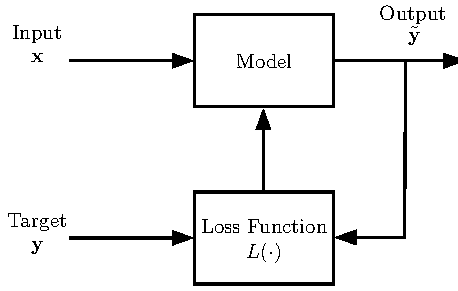
\includegraphics[width=0.5\textwidth]{sup_learning_schematic}
	\caption{Simplified Supervised Learning Schematic}
	\label{fig:sup_learning}
\end{figure}

\subsection{Unsupervised Learning}\label{sec:unsup_learning}

Contrary to the aforementioned Supervised Learning method, Unsupervised Learning does not have a well specified "target" and therefore the model now has a different purpose, to create some sort of structure based solely on the inputs and the relationships between them. Unsupervised Learning typically translates to clustering.

Clustering is the action of grouping together inputs that have some degree of similarity, for instance, trying to separate different animals by the number of legs they possess, or which environment they reside is a type of unsupervised clustering since it depends only on the characteristics of the input data. A good example of this approach is recommendation systems.


\section{Artificial Neural Networks} \label{sec:ann}

What mainly highlights our species is the seemingly unending capacity to learn and adapt. The organ responsible for such, the brain has been subjected to 

Over the years, several studies (?????) have been published on the brain and its composition although several things are still undiscovered or undetermined.

The brain is the most complex organ in the human body and hosts $10$ to $20$ billion neurons, its main component. These neurons (Figure \ref{fig:neurons}) are physically connected through its dendrites and axons, these connections are susceptible to electrical impulses called synapses, most neural cells send signals through the axons and receive them from the dendrites.

\begin{figure}[H]
	\centering
    \def\svgwidth{0.6\columnwidth}
	%LaTeX with PSTricks extensions
%%Creator: inkscape 0.92.3
%%Please note this file requires PSTricks extensions
\psset{xunit=.5pt,yunit=.5pt,runit=.5pt}
\begin{pspicture}(399.8210144,214.97999573)
{
\newrgbcolor{curcolor}{0.68627453 0.63921571 0.81176472}
\pscustom[linestyle=none,fillstyle=solid,fillcolor=curcolor]
{
\newpath
\moveto(126.833,82.89099573)
\curveto(130.439,84.38199573)(127.833,89.22399573)(127.833,89.22399573)
\curveto(127.833,89.22399573)(101.5,94.22399573)(106.833,113.22399573)
\lineto(112.166,132.22399573)
\curveto(112.166,132.22399573)(118.499,136.89199573)(123.833,140.55799573)
\curveto(129.167,144.22399573)(127.5,145.55699573)(123.166,144.22399573)
\curveto(122.499,145.55799573)(125.499,148.89099573)(125.833,149.55699573)
\curveto(126.166,150.22499573)(131.833,162.55799573)(120.5,145.89099573)
\curveto(120.5,144.89099573)(110.833,133.89099573)(116.5,153.55699573)
\curveto(116.5,153.55699573)(123.833,188.89099573)(115.5,163.22499573)
\curveto(115.5,163.22499573)(113.5,156.89099573)(111.5,161.22499573)
\curveto(111.5,161.22499573)(115.5,147.88999573)(103.167,115.22399573)
\curveto(100.167,117.89099573)(98.167,120.55799573)(98.167,120.55799573)
\curveto(97.167,122.22399573)(96.5,126.22399573)(101.167,134.89099573)
\curveto(105.834,143.55799573)(108.5,148.89099573)(108.5,148.89099573)
\curveto(108.5,148.89099573)(112.833,157.22499573)(107.5,151.22499573)
\curveto(107.5,151.22499573)(107.833,170.22399573)(104.5,146.89099573)
\curveto(104.5,146.89099573)(101.834,142.88999573)(100.167,141.22399573)
\curveto(100.167,141.22399573)(104.834,152.22399573)(99.167,149.55699573)
\curveto(99.167,149.55699573)(96.167,156.55699573)(96.5,148.55699573)
\curveto(96.833,140.55799573)(98.5,138.88999573)(97.5,134.22399573)
\curveto(96.5,129.55799573)(94.833,131.55799573)(94.5,135.55799573)
\curveto(94.167,139.55799573)(84.5,135.22399573)(99.833,110.89099573)
\curveto(99.833,110.89099573)(105.166,85.55799573)(85.5,103.55799573)
\curveto(85.5,103.55799573)(60.833,123.22499573)(92.5,146.55799573)
\curveto(88.5,143.55799573)(86.833,140.22299573)(87.5,144.22399573)
\curveto(88.167,148.22499573)(87.5,147.89099573)(87.5,147.89099573)
\curveto(87.5,147.89099573)(83.833,140.88999573)(81.5,139.22399573)
\curveto(79.167,137.55799573)(69.833,134.55699573)(90.5,157.89099573)
\curveto(86.5,154.89099573)(79.167,149.22399573)(86.5,165.55799573)
\curveto(79.5,154.55799573)(75.167,141.89099573)(71.167,152.89099573)
\curveto(71.167,152.89099573)(75.5,106.55899573)(65.167,136.55799573)
\curveto(65.167,136.55799573)(61.5,142.55799573)(70.167,172.22499573)
\curveto(67.167,165.55799573)(64.5,156.22499573)(65.167,175.55799573)
\curveto(65.167,175.55799573)(62.167,174.55799573)(62.834,153.22499573)
\curveto(62.834,153.22499573)(53.501,131.89099573)(55.501,160.22499573)
\curveto(55.501,160.22499573)(58.501,172.89099573)(58.834,175.22499573)
\curveto(59.167,177.55899573)(57.167,174.55799573)(56.501,173.22499573)
\curveto(55.835,171.89199573)(55.834,178.22499573)(55.834,178.22499573)
\curveto(55.834,178.22499573)(53.834,175.22499573)(53.501,171.22499573)
\curveto(53.168,167.22499573)(50.168,174.22499573)(49.168,175.89199573)
\curveto(48.168,177.55899573)(55.834,164.89199573)(50.501,154.22599573)
\curveto(50.501,154.22599573)(42.835,166.89199573)(42.168,163.22599573)
\curveto(41.501,159.55899573)(58.168,139.55799573)(58.501,138.22499573)
\curveto(58.834,136.89199573)(68.501,127.22499573)(56.501,128.89199573)
\curveto(52.501,129.22499573)(50.168,131.55899573)(48.168,134.89199573)
\curveto(46.168,138.22499573)(41.835,144.89199573)(41.835,144.89199573)
\lineto(32.168,155.89199573)
\lineto(31.5,171.22499573)
\lineto(30.167,167.55799573)
\lineto(27.834,169.89099573)
\lineto(29.834,165.22399573)
\lineto(30.167,158.89099573)
\lineto(27.834,157.89099573)
\curveto(27.834,157.89099573)(55.834,129.55699573)(33.167,140.22399573)
\curveto(33.167,140.22399573)(24.833,137.88999573)(43.5,133.22399573)
\curveto(43.5,133.22399573)(44.833,125.55799573)(60.833,124.55799573)
\curveto(60.833,124.55799573)(72.833,111.55699573)(75.833,99.22399573)
\curveto(75.833,99.22399573)(79.166,72.55699573)(63.833,93.22399573)
\curveto(63.833,93.22399573)(66.833,85.89099573)(64.833,85.89099573)
\curveto(62.833,85.89099573)(53.166,91.55799573)(51.833,91.55799573)
\curveto(50.5,91.55799573)(46.5,89.55799573)(46.5,89.55799573)
\curveto(46.5,89.55799573)(73.5,82.89199573)(48.167,82.55799573)
\curveto(48.167,82.55799573)(30.167,76.22499573)(37.167,118.55799573)
\curveto(37.167,118.55799573)(34.834,106.22399573)(32.834,117.89099573)
\curveto(32.834,117.89099573)(27.501,91.55699573)(32.834,81.22399573)
\curveto(32.834,81.22399573)(37.834,74.89199573)(30.501,74.55799573)
\curveto(30.501,74.55799573)(39.501,75.89199573)(48.501,78.55799573)
\curveto(48.501,78.55799573)(41.834,65.22399573)(38.501,65.22399573)
\curveto(38.501,65.22399573)(41.501,64.55799573)(38.168,62.55799573)
\curveto(38.168,62.55799573)(39.501,59.89199573)(43.168,64.55799573)
\curveto(46.835,69.22399573)(52.168,80.55699573)(65.168,80.22399573)
\curveto(69.501,78.89099573)(85.501,65.55799573)(61.168,60.89099573)
\curveto(53.835,57.89099573)(26.168,47.88999573)(28.501,46.22399573)
\curveto(30.834,44.55799573)(44.834,54.55799573)(42.501,49.55799573)
\curveto(40.168,44.55799573)(32.501,30.22399573)(32.501,30.22399573)
\curveto(32.501,30.22399573)(41.834,51.55699573)(39.834,35.22399573)
\curveto(40.834,33.89099573)(65.167,80.55699573)(47.834,35.22399573)
\curveto(48.167,34.22399573)(52.167,41.22499573)(52.834,31.89099573)
\curveto(52.834,31.89099573)(53.167,67.22299573)(78.167,56.55699573)
\curveto(78.834,47.55699573)(73.5,35.22499573)(59.5,26.89099573)
\curveto(73.833,35.22399573)(76.167,38.89099573)(69.5,24.89099573)
\curveto(72.833,28.22399573)(74.5,27.88999573)(75.5,23.55699573)
\curveto(76.833,38.55699573)(79.5,43.22299573)(82.167,45.55699573)
\curveto(84.834,38.55699573)(85.834,35.55799573)(86.167,33.89099573)
\curveto(86.5,32.22399573)(84.5,57.55799573)(84.167,58.89099573)
\curveto(83.834,60.22399573)(97.167,59.55699573)(97.167,59.55699573)
\curveto(97.167,59.55699573)(107.167,40.22299573)(102.834,31.55699573)
\curveto(105.167,38.89099573)(101.167,53.55799573)(118.834,27.89099573)
\curveto(118.834,27.89099573)(106.834,41.22399573)(126.167,36.22399573)
\curveto(119.5,41.55699573)(107.167,48.88999573)(103.834,54.55699573)
\curveto(100.501,60.22399573)(99.834,67.88999573)(110.167,60.55699573)
\curveto(120.5,53.22399573)(126.834,50.22499573)(127.834,50.89099573)
\curveto(128.834,51.55699573)(108.167,60.89099573)(131.167,56.89099573)
\curveto(116.5,63.22399573)(92.167,68.55799573)(126.833,82.89099573)
\closepath
}
}
{
\newrgbcolor{curcolor}{0 0 0}
\pscustom[linewidth=1,linecolor=curcolor]
{
\newpath
\moveto(126.833,82.89099573)
\curveto(130.439,84.38199573)(127.833,89.22399573)(127.833,89.22399573)
\curveto(127.833,89.22399573)(101.5,94.22399573)(106.833,113.22399573)
\lineto(112.166,132.22399573)
\curveto(112.166,132.22399573)(118.499,136.89199573)(123.833,140.55799573)
\curveto(129.167,144.22399573)(127.5,145.55699573)(123.166,144.22399573)
\curveto(122.499,145.55799573)(125.499,148.89099573)(125.833,149.55699573)
\curveto(126.166,150.22499573)(131.833,162.55799573)(120.5,145.89099573)
\curveto(120.5,144.89099573)(110.833,133.89099573)(116.5,153.55699573)
\curveto(116.5,153.55699573)(123.833,188.89099573)(115.5,163.22499573)
\curveto(115.5,163.22499573)(113.5,156.89099573)(111.5,161.22499573)
\curveto(111.5,161.22499573)(115.5,147.88999573)(103.167,115.22399573)
\curveto(100.167,117.89099573)(98.167,120.55799573)(98.167,120.55799573)
\curveto(97.167,122.22399573)(96.5,126.22399573)(101.167,134.89099573)
\curveto(105.834,143.55799573)(108.5,148.89099573)(108.5,148.89099573)
\curveto(108.5,148.89099573)(112.833,157.22499573)(107.5,151.22499573)
\curveto(107.5,151.22499573)(107.833,170.22399573)(104.5,146.89099573)
\curveto(104.5,146.89099573)(101.834,142.88999573)(100.167,141.22399573)
\curveto(100.167,141.22399573)(104.834,152.22399573)(99.167,149.55699573)
\curveto(99.167,149.55699573)(96.167,156.55699573)(96.5,148.55699573)
\curveto(96.833,140.55799573)(98.5,138.88999573)(97.5,134.22399573)
\curveto(96.5,129.55799573)(94.833,131.55799573)(94.5,135.55799573)
\curveto(94.167,139.55799573)(84.5,135.22399573)(99.833,110.89099573)
\curveto(99.833,110.89099573)(105.166,85.55799573)(85.5,103.55799573)
\curveto(85.5,103.55799573)(60.833,123.22499573)(92.5,146.55799573)
\curveto(88.5,143.55799573)(86.833,140.22299573)(87.5,144.22399573)
\curveto(88.167,148.22499573)(87.5,147.89099573)(87.5,147.89099573)
\curveto(87.5,147.89099573)(83.833,140.88999573)(81.5,139.22399573)
\curveto(79.167,137.55799573)(69.833,134.55699573)(90.5,157.89099573)
\curveto(86.5,154.89099573)(79.167,149.22399573)(86.5,165.55799573)
\curveto(79.5,154.55799573)(75.167,141.89099573)(71.167,152.89099573)
\curveto(71.167,152.89099573)(75.5,106.55899573)(65.167,136.55799573)
\curveto(65.167,136.55799573)(61.5,142.55799573)(70.167,172.22499573)
\curveto(67.167,165.55799573)(64.5,156.22499573)(65.167,175.55799573)
\curveto(65.167,175.55799573)(62.167,174.55799573)(62.834,153.22499573)
\curveto(62.834,153.22499573)(53.501,131.89099573)(55.501,160.22499573)
\curveto(55.501,160.22499573)(58.501,172.89099573)(58.834,175.22499573)
\curveto(59.167,177.55899573)(57.167,174.55799573)(56.501,173.22499573)
\curveto(55.835,171.89199573)(55.834,178.22499573)(55.834,178.22499573)
\curveto(55.834,178.22499573)(53.834,175.22499573)(53.501,171.22499573)
\curveto(53.168,167.22499573)(50.168,174.22499573)(49.168,175.89199573)
\curveto(48.168,177.55899573)(55.834,164.89199573)(50.501,154.22599573)
\curveto(50.501,154.22599573)(42.835,166.89199573)(42.168,163.22599573)
\curveto(41.501,159.55899573)(58.168,139.55799573)(58.501,138.22499573)
\curveto(58.834,136.89199573)(68.501,127.22499573)(56.501,128.89199573)
\curveto(52.501,129.22499573)(50.168,131.55899573)(48.168,134.89199573)
\curveto(46.168,138.22499573)(41.835,144.89199573)(41.835,144.89199573)
\lineto(32.168,155.89199573)
\lineto(31.5,171.22499573)
\lineto(30.167,167.55799573)
\lineto(27.834,169.89099573)
\lineto(29.834,165.22399573)
\lineto(30.167,158.89099573)
\lineto(27.834,157.89099573)
\curveto(27.834,157.89099573)(55.834,129.55699573)(33.167,140.22399573)
\curveto(33.167,140.22399573)(24.833,137.88999573)(43.5,133.22399573)
\curveto(43.5,133.22399573)(44.833,125.55799573)(60.833,124.55799573)
\curveto(60.833,124.55799573)(72.833,111.55699573)(75.833,99.22399573)
\curveto(75.833,99.22399573)(79.166,72.55699573)(63.833,93.22399573)
\curveto(63.833,93.22399573)(66.833,85.89099573)(64.833,85.89099573)
\curveto(62.833,85.89099573)(53.166,91.55799573)(51.833,91.55799573)
\curveto(50.5,91.55799573)(46.5,89.55799573)(46.5,89.55799573)
\curveto(46.5,89.55799573)(73.5,82.89199573)(48.167,82.55799573)
\curveto(48.167,82.55799573)(30.167,76.22499573)(37.167,118.55799573)
\curveto(37.167,118.55799573)(34.834,106.22399573)(32.834,117.89099573)
\curveto(32.834,117.89099573)(27.501,91.55699573)(32.834,81.22399573)
\curveto(32.834,81.22399573)(37.834,74.89199573)(30.501,74.55799573)
\curveto(30.501,74.55799573)(39.501,75.89199573)(48.501,78.55799573)
\curveto(48.501,78.55799573)(41.834,65.22399573)(38.501,65.22399573)
\curveto(38.501,65.22399573)(41.501,64.55799573)(38.168,62.55799573)
\curveto(38.168,62.55799573)(39.501,59.89199573)(43.168,64.55799573)
\curveto(46.835,69.22399573)(52.168,80.55699573)(65.168,80.22399573)
\curveto(69.501,78.89099573)(85.501,65.55799573)(61.168,60.89099573)
\curveto(53.835,57.89099573)(26.168,47.88999573)(28.501,46.22399573)
\curveto(30.834,44.55799573)(44.834,54.55799573)(42.501,49.55799573)
\curveto(40.168,44.55799573)(32.501,30.22399573)(32.501,30.22399573)
\curveto(32.501,30.22399573)(41.834,51.55699573)(39.834,35.22399573)
\curveto(40.834,33.89099573)(65.167,80.55699573)(47.834,35.22399573)
\curveto(48.167,34.22399573)(52.167,41.22499573)(52.834,31.89099573)
\curveto(52.834,31.89099573)(53.167,67.22299573)(78.167,56.55699573)
\curveto(78.834,47.55699573)(73.5,35.22499573)(59.5,26.89099573)
\curveto(73.833,35.22399573)(76.167,38.89099573)(69.5,24.89099573)
\curveto(72.833,28.22399573)(74.5,27.88999573)(75.5,23.55699573)
\curveto(76.833,38.55699573)(79.5,43.22299573)(82.167,45.55699573)
\curveto(84.834,38.55699573)(85.834,35.55799573)(86.167,33.89099573)
\curveto(86.5,32.22399573)(84.5,57.55799573)(84.167,58.89099573)
\curveto(83.834,60.22399573)(97.167,59.55699573)(97.167,59.55699573)
\curveto(97.167,59.55699573)(107.167,40.22299573)(102.834,31.55699573)
\curveto(105.167,38.89099573)(101.167,53.55799573)(118.834,27.89099573)
\curveto(118.834,27.89099573)(106.834,41.22399573)(126.167,36.22399573)
\curveto(119.5,41.55699573)(107.167,48.88999573)(103.834,54.55699573)
\curveto(100.501,60.22399573)(99.834,67.88999573)(110.167,60.55699573)
\curveto(120.5,53.22399573)(126.834,50.22499573)(127.834,50.89099573)
\curveto(128.834,51.55699573)(108.167,60.89099573)(131.167,56.89099573)
\curveto(116.5,63.22399573)(92.167,68.55799573)(126.833,82.89099573)
\closepath
}
}
{
\newrgbcolor{curcolor}{0.35686275 0.60000002 0.45490196}
\pscustom[linestyle=none,fillstyle=solid,fillcolor=curcolor]
{
\newpath
\moveto(85.125,78.39099573)
\curveto(85,82.89099573)(86.5,84.26599573)(89.25,83.89099573)
\curveto(92,83.51599573)(94.75,82.26599573)(95.875,81.01599573)
\curveto(97,79.76599573)(98.625,77.51599573)(98.875,76.64099573)
\curveto(99.125,75.76599573)(99.25,74.89099573)(99.375,74.01599573)
\curveto(99.5,73.14099573)(99.875,72.26599573)(99.5,71.51599573)
\curveto(99.125,70.76599573)(98.625,69.14099573)(97.625,69.01599573)
\curveto(96.625,68.89099573)(96,68.64099573)(94.875,69.26599573)
\curveto(93.75,69.89099573)(92,71.01599573)(91.25,71.64099573)
\curveto(90.5,72.26599573)(87.5,75.26599573)(86.875,76.14099573)
\curveto(86.25,77.01599573)(85.125,78.39099573)(85.125,78.39099573)
\closepath
}
}
{
\newrgbcolor{curcolor}{0 0 0}
\pscustom[linewidth=1,linecolor=curcolor]
{
\newpath
\moveto(85.125,78.39099573)
\curveto(85,82.89099573)(86.5,84.26599573)(89.25,83.89099573)
\curveto(92,83.51599573)(94.75,82.26599573)(95.875,81.01599573)
\curveto(97,79.76599573)(98.625,77.51599573)(98.875,76.64099573)
\curveto(99.125,75.76599573)(99.25,74.89099573)(99.375,74.01599573)
\curveto(99.5,73.14099573)(99.875,72.26599573)(99.5,71.51599573)
\curveto(99.125,70.76599573)(98.625,69.14099573)(97.625,69.01599573)
\curveto(96.625,68.89099573)(96,68.64099573)(94.875,69.26599573)
\curveto(93.75,69.89099573)(92,71.01599573)(91.25,71.64099573)
\curveto(90.5,72.26599573)(87.5,75.26599573)(86.875,76.14099573)
\curveto(86.25,77.01599573)(85.125,78.39099573)(85.125,78.39099573)
\closepath
}
}
{
\newrgbcolor{curcolor}{0.97647059 0.83529413 0.40000001}
\pscustom[linestyle=none,fillstyle=solid,fillcolor=curcolor]
{
\newpath
\moveto(127.5,81.64099573)
\curveto(129.75,86.14099573)(129.125,87.64099573)(128.625,89.01599573)
\curveto(128.125,90.39099573)(146.25,91.01599573)(158.625,84.01599573)
\curveto(158.625,84.01599573)(170.375,80.01599573)(159.875,72.51599573)
\curveto(159.875,72.51599573)(140.375,69.64099573)(127.5,81.64099573)
\closepath
}
}
{
\newrgbcolor{curcolor}{0 0 0}
\pscustom[linewidth=1,linecolor=curcolor]
{
\newpath
\moveto(127.5,81.64099573)
\curveto(129.75,86.14099573)(129.125,87.64099573)(128.625,89.01599573)
\curveto(128.125,90.39099573)(146.25,91.01599573)(158.625,84.01599573)
\curveto(158.625,84.01599573)(170.375,80.01599573)(159.875,72.51599573)
\curveto(159.875,72.51599573)(140.375,69.64099573)(127.5,81.64099573)
\closepath
}
}
{
\newrgbcolor{curcolor}{0.97647059 0.83529413 0.40000001}
\pscustom[linestyle=none,fillstyle=solid,fillcolor=curcolor]
{
\newpath
\moveto(168.375,69.14099573)
\curveto(168.375,69.14099573)(164.75,70.89099573)(165.875,74.14099573)
\curveto(167,77.39099573)(168,77.39099573)(169,77.76599573)
\curveto(170,78.14099573)(175.75,78.01599573)(176.25,78.01599573)
\curveto(176.75,78.01599573)(196,76.01599573)(198.625,73.76599573)
\curveto(201.25,71.51599573)(202.125,68.76599573)(202.125,67.64099573)
\curveto(202.125,66.51599573)(201.875,62.89099573)(198.375,62.89099573)
\curveto(194.875,62.89099573)(180,63.14099573)(179.375,63.76599573)
\curveto(178.75,64.39099573)(170.875,66.51599573)(168.375,69.14099573)
\closepath
}
}
{
\newrgbcolor{curcolor}{0 0 0}
\pscustom[linewidth=1,linecolor=curcolor]
{
\newpath
\moveto(168.375,69.14099573)
\curveto(168.375,69.14099573)(164.75,70.89099573)(165.875,74.14099573)
\curveto(167,77.39099573)(168,77.39099573)(169,77.76599573)
\curveto(170,78.14099573)(175.75,78.01599573)(176.25,78.01599573)
\curveto(176.75,78.01599573)(196,76.01599573)(198.625,73.76599573)
\curveto(201.25,71.51599573)(202.125,68.76599573)(202.125,67.64099573)
\curveto(202.125,66.51599573)(201.875,62.89099573)(198.375,62.89099573)
\curveto(194.875,62.89099573)(180,63.14099573)(179.375,63.76599573)
\curveto(178.75,64.39099573)(170.875,66.51599573)(168.375,69.14099573)
\closepath
}
}
{
\newrgbcolor{curcolor}{0.97647059 0.83529413 0.40000001}
\pscustom[linestyle=none,fillstyle=solid,fillcolor=curcolor]
{
\newpath
\moveto(214.375,59.89099573)
\curveto(207.75,62.01599573)(204.875,64.51599573)(205.125,67.14099573)
\curveto(205.375,69.76599573)(205.875,70.76599573)(207,71.39099573)
\curveto(208.125,72.01599573)(210.875,72.76599573)(211.625,73.01599573)
\curveto(212.375,73.26599573)(234,76.39099573)(236.125,75.89099573)
\curveto(238.25,75.39099573)(240.875,72.89099573)(241.125,71.39099573)
\curveto(241.375,69.89099573)(243.75,66.39099573)(238.375,64.14099573)
\curveto(233,61.89099573)(229,60.39099573)(225.375,60.14099573)
\curveto(221.75,59.89099573)(214.375,59.89099573)(214.375,59.89099573)
\closepath
}
}
{
\newrgbcolor{curcolor}{0 0 0}
\pscustom[linewidth=1,linecolor=curcolor]
{
\newpath
\moveto(214.375,59.89099573)
\curveto(207.75,62.01599573)(204.875,64.51599573)(205.125,67.14099573)
\curveto(205.375,69.76599573)(205.875,70.76599573)(207,71.39099573)
\curveto(208.125,72.01599573)(210.875,72.76599573)(211.625,73.01599573)
\curveto(212.375,73.26599573)(234,76.39099573)(236.125,75.89099573)
\curveto(238.25,75.39099573)(240.875,72.89099573)(241.125,71.39099573)
\curveto(241.375,69.89099573)(243.75,66.39099573)(238.375,64.14099573)
\curveto(233,61.89099573)(229,60.39099573)(225.375,60.14099573)
\curveto(221.75,59.89099573)(214.375,59.89099573)(214.375,59.89099573)
\closepath
}
}
{
\newrgbcolor{curcolor}{0.97647059 0.83529413 0.40000001}
\pscustom[linestyle=none,fillstyle=solid,fillcolor=curcolor]
{
\newpath
\moveto(252.125,69.51599573)
\curveto(246.116,69.13999573)(244.25,68.39099573)(244.375,72.89099573)
\curveto(244.5,77.39099573)(244,79.01599573)(247.625,80.76599573)
\curveto(251.25,82.51599573)(261.5,89.26599573)(263.125,90.01599573)
\curveto(264.75,90.76599573)(270,92.39099573)(272.375,89.26599573)
\curveto(274.75,86.14099573)(274.5,84.76599573)(272,82.01599573)
\curveto(269.5,79.26599573)(256.125,69.76599573)(252.125,69.51599573)
\closepath
}
}
{
\newrgbcolor{curcolor}{0 0 0}
\pscustom[linewidth=1,linecolor=curcolor]
{
\newpath
\moveto(252.125,69.51599573)
\curveto(246.116,69.13999573)(244.25,68.39099573)(244.375,72.89099573)
\curveto(244.5,77.39099573)(244,79.01599573)(247.625,80.76599573)
\curveto(251.25,82.51599573)(261.5,89.26599573)(263.125,90.01599573)
\curveto(264.75,90.76599573)(270,92.39099573)(272.375,89.26599573)
\curveto(274.75,86.14099573)(274.5,84.76599573)(272,82.01599573)
\curveto(269.5,79.26599573)(256.125,69.76599573)(252.125,69.51599573)
\closepath
}
}
{
\newrgbcolor{curcolor}{0.97647059 0.83529413 0.40000001}
\pscustom[linestyle=none,fillstyle=solid,fillcolor=curcolor]
{
\newpath
\moveto(274,92.14099573)
\curveto(271.56,96.67299573)(270.625,99.14099573)(272.875,102.39099573)
\curveto(275.125,105.64099573)(286,121.14099573)(286.375,121.64099573)
\curveto(286.75,122.14099573)(291,124.01599573)(294.75,120.76599573)
\curveto(298.5,117.51599573)(299.25,115.26599573)(295.75,110.51599573)
\curveto(292.25,105.76599573)(284.125,93.01599573)(281.25,91.51599573)
\curveto(278.375,90.01599573)(275.75,88.89099573)(274,92.14099573)
\closepath
}
}
{
\newrgbcolor{curcolor}{0 0 0}
\pscustom[linewidth=1,linecolor=curcolor]
{
\newpath
\moveto(274,92.14099573)
\curveto(271.56,96.67299573)(270.625,99.14099573)(272.875,102.39099573)
\curveto(275.125,105.64099573)(286,121.14099573)(286.375,121.64099573)
\curveto(286.75,122.14099573)(291,124.01599573)(294.75,120.76599573)
\curveto(298.5,117.51599573)(299.25,115.26599573)(295.75,110.51599573)
\curveto(292.25,105.76599573)(284.125,93.01599573)(281.25,91.51599573)
\curveto(278.375,90.01599573)(275.75,88.89099573)(274,92.14099573)
\closepath
}
}
{
\newrgbcolor{curcolor}{0.90196079 0.54509807 0.3764706}
\pscustom[linestyle=none,fillstyle=solid,fillcolor=curcolor]
{
\newpath
\moveto(143.375,84.01599121)
\curveto(143.375,82.84238612)(141.86396103,81.89099121)(140,81.89099121)
\curveto(138.13603897,81.89099121)(136.625,82.84238612)(136.625,84.01599121)
\curveto(136.625,85.1895963)(138.13603897,86.14099121)(140,86.14099121)
\curveto(141.86396103,86.14099121)(143.375,85.1895963)(143.375,84.01599121)
\closepath
}
}
{
\newrgbcolor{curcolor}{0.71764708 0.3882353 0.15686275}
\pscustom[linewidth=1,linecolor=curcolor]
{
\newpath
\moveto(143.375,84.01599121)
\curveto(143.375,82.84238612)(141.86396103,81.89099121)(140,81.89099121)
\curveto(138.13603897,81.89099121)(136.625,82.84238612)(136.625,84.01599121)
\curveto(136.625,85.1895963)(138.13603897,86.14099121)(140,86.14099121)
\curveto(141.86396103,86.14099121)(143.375,85.1895963)(143.375,84.01599121)
\closepath
}
}
{
\newrgbcolor{curcolor}{0.90196079 0.54509807 0.3764706}
\pscustom[linestyle=none,fillstyle=solid,fillcolor=curcolor]
{
\newpath
\moveto(185.25,70.14099121)
\curveto(185.25,68.96738612)(183.73896103,68.01599121)(181.875,68.01599121)
\curveto(180.01103897,68.01599121)(178.5,68.96738612)(178.5,70.14099121)
\curveto(178.5,71.3145963)(180.01103897,72.26599121)(181.875,72.26599121)
\curveto(183.73896103,72.26599121)(185.25,71.3145963)(185.25,70.14099121)
\closepath
}
}
{
\newrgbcolor{curcolor}{0.71764708 0.3882353 0.15686275}
\pscustom[linewidth=1,linecolor=curcolor]
{
\newpath
\moveto(185.25,70.14099121)
\curveto(185.25,68.96738612)(183.73896103,68.01599121)(181.875,68.01599121)
\curveto(180.01103897,68.01599121)(178.5,68.96738612)(178.5,70.14099121)
\curveto(178.5,71.3145963)(180.01103897,72.26599121)(181.875,72.26599121)
\curveto(183.73896103,72.26599121)(185.25,71.3145963)(185.25,70.14099121)
\closepath
}
}
{
\newrgbcolor{curcolor}{0.90196079 0.54509807 0.3764706}
\pscustom[linestyle=none,fillstyle=solid,fillcolor=curcolor]
{
\newpath
\moveto(227.5,67.14099121)
\curveto(227.5,65.96738612)(225.98896103,65.01599121)(224.125,65.01599121)
\curveto(222.26103897,65.01599121)(220.75,65.96738612)(220.75,67.14099121)
\curveto(220.75,68.3145963)(222.26103897,69.26599121)(224.125,69.26599121)
\curveto(225.98896103,69.26599121)(227.5,68.3145963)(227.5,67.14099121)
\closepath
}
}
{
\newrgbcolor{curcolor}{0.71764708 0.3882353 0.15686275}
\pscustom[linewidth=1,linecolor=curcolor]
{
\newpath
\moveto(227.5,67.14099121)
\curveto(227.5,65.96738612)(225.98896103,65.01599121)(224.125,65.01599121)
\curveto(222.26103897,65.01599121)(220.75,65.96738612)(220.75,67.14099121)
\curveto(220.75,68.3145963)(222.26103897,69.26599121)(224.125,69.26599121)
\curveto(225.98896103,69.26599121)(227.5,68.3145963)(227.5,67.14099121)
\closepath
}
}
{
\newrgbcolor{curcolor}{0.90196079 0.54509807 0.3764706}
\pscustom[linestyle=none,fillstyle=solid,fillcolor=curcolor]
{
\newpath
\moveto(261.59140605,82.15423611)
\curveto(262.07293622,81.08390826)(261.08522601,79.59625682)(259.38529355,78.83147361)
\curveto(257.68536109,78.0666904)(255.91693622,78.31438326)(255.43540605,79.38471111)
\curveto(254.95387588,80.45503895)(255.94158609,81.9426904)(257.64151855,82.70747361)
\curveto(259.34145101,83.47225682)(261.10987588,83.22456395)(261.59140605,82.15423611)
\closepath
}
}
{
\newrgbcolor{curcolor}{0.71764708 0.3882353 0.15686275}
\pscustom[linewidth=1.00004504,linecolor=curcolor]
{
\newpath
\moveto(261.59140605,82.15423611)
\curveto(262.07293622,81.08390826)(261.08522601,79.59625682)(259.38529355,78.83147361)
\curveto(257.68536109,78.0666904)(255.91693622,78.31438326)(255.43540605,79.38471111)
\curveto(254.95387588,80.45503895)(255.94158609,81.9426904)(257.64151855,82.70747361)
\curveto(259.34145101,83.47225682)(261.10987588,83.22456395)(261.59140605,82.15423611)
\closepath
}
}
{
\newrgbcolor{curcolor}{0.90196079 0.54509807 0.3764706}
\pscustom[linestyle=none,fillstyle=solid,fillcolor=curcolor]
{
\newpath
\moveto(285.44565018,110.34331662)
\curveto(286.43171318,109.70698793)(286.41178986,107.92156667)(285.40115018,106.35546662)
\curveto(284.39051051,104.78936656)(282.77186318,104.03563793)(281.78580018,104.67196662)
\curveto(280.79973719,105.3082953)(280.81966051,107.09371656)(281.83030018,108.65981662)
\curveto(282.84093986,110.22591667)(284.45958719,110.9796453)(285.44565018,110.34331662)
\closepath
}
}
{
\newrgbcolor{curcolor}{0.71764708 0.3882353 0.15686275}
\pscustom[linewidth=0.99995844,linecolor=curcolor]
{
\newpath
\moveto(285.44565018,110.34331662)
\curveto(286.43171318,109.70698793)(286.41178986,107.92156667)(285.40115018,106.35546662)
\curveto(284.39051051,104.78936656)(282.77186318,104.03563793)(281.78580018,104.67196662)
\curveto(280.79973719,105.3082953)(280.81966051,107.09371656)(281.83030018,108.65981662)
\curveto(282.84093986,110.22591667)(284.45958719,110.9796453)(285.44565018,110.34331662)
\closepath
}
}
{
\newrgbcolor{curcolor}{0.68627453 0.63921571 0.81176472}
\pscustom[linestyle=none,fillstyle=solid,fillcolor=curcolor]
{
\newpath
\moveto(164.25,77.89099573)
\curveto(166.5,77.39099573)(168,77.39099573)(168,77.39099573)
\lineto(165.875,74.14099573)
\lineto(161.75,74.26599573)
\closepath
}
}
{
\newrgbcolor{curcolor}{0 0 0}
\pscustom[linewidth=1,linecolor=curcolor]
{
\newpath
\moveto(164.25,77.89099573)
\curveto(166.5,77.39099573)(168,77.39099573)(168,77.39099573)
\lineto(165.875,74.14099573)
\lineto(161.75,74.26599573)
\closepath
}
}
{
\newrgbcolor{curcolor}{0.68627453 0.63921571 0.81176472}
\pscustom[linestyle=none,fillstyle=solid,fillcolor=curcolor]
{
\newpath
\moveto(201.75,69.76599573)
\lineto(205.875,70.01599573)
\lineto(205,65.89099573)
\lineto(201.875,65.89099573)
\curveto(201.875,65.89099573)(202.125,69.26599573)(201.75,69.76599573)
\closepath
}
}
{
\newrgbcolor{curcolor}{0 0 0}
\pscustom[linewidth=1,linecolor=curcolor]
{
\newpath
\moveto(201.75,69.76599573)
\lineto(205.875,70.01599573)
\lineto(205,65.89099573)
\lineto(201.875,65.89099573)
\curveto(201.875,65.89099573)(202.125,69.26599573)(201.75,69.76599573)
\closepath
}
}
{
\newrgbcolor{curcolor}{0.68627453 0.63921571 0.81176472}
\pscustom[linestyle=none,fillstyle=solid,fillcolor=curcolor]
{
\newpath
\moveto(240.25,73.39099573)
\curveto(240.25,73.39099573)(243.625,75.89099573)(243.875,76.51599573)
\curveto(244.125,77.14099573)(244.25,71.51599573)(244.375,71.14099573)
\curveto(244.5,70.76599573)(242.125,70.26599573)(242.125,70.26599573)
\closepath
}
}
{
\newrgbcolor{curcolor}{0 0 0}
\pscustom[linewidth=1,linecolor=curcolor]
{
\newpath
\moveto(240.25,73.39099573)
\curveto(240.25,73.39099573)(243.625,75.89099573)(243.875,76.51599573)
\curveto(244.125,77.14099573)(244.25,71.51599573)(244.375,71.14099573)
\curveto(244.5,70.76599573)(242.125,70.26599573)(242.125,70.26599573)
\closepath
}
}
{
\newrgbcolor{curcolor}{0.68627453 0.63921571 0.81176472}
\pscustom[linestyle=none,fillstyle=solid,fillcolor=curcolor]
{
\newpath
\moveto(269.625,91.26599573)
\lineto(272.375,95.14099573)
\lineto(275.25,90.76599573)
\lineto(273.25,88.89099573)
\curveto(273.25,88.89099573)(271.5,91.01599573)(269.625,91.26599573)
\closepath
}
}
{
\newrgbcolor{curcolor}{0 0 0}
\pscustom[linewidth=1,linecolor=curcolor]
{
\newpath
\moveto(269.625,91.26599573)
\lineto(272.375,95.14099573)
\lineto(275.25,90.76599573)
\lineto(273.25,88.89099573)
\curveto(273.25,88.89099573)(271.5,91.01599573)(269.625,91.26599573)
\closepath
}
}
{
\newrgbcolor{curcolor}{0.68627453 0.63921571 0.81176472}
\pscustom[linestyle=none,fillstyle=solid,fillcolor=curcolor]
{
\newpath
\moveto(291.167,122.72399573)
\lineto(291.29,122.99399573)
\curveto(294.565,130.24499573)(297.184,137.76599573)(298.5,141.05799573)
\curveto(299.833,144.39099573)(300.333,152.22399573)(299.833,153.05799573)
\curveto(299.333,153.89199573)(297.833,159.55799573)(294,158.39099573)
\curveto(290.167,157.22399573)(291.499,158.39099573)(290.333,156.55799573)
\curveto(289.167,154.72499573)(286.334,154.55799573)(286.167,156.22499573)
\curveto(286,157.89199573)(286.667,158.39199573)(289.5,158.89199573)
\curveto(292.333,159.39199573)(290.833,161.39199573)(288.833,163.22499573)
\curveto(286.833,165.05799573)(281.499,165.05799573)(285.333,167.55799573)
\curveto(289.167,170.05799573)(289.333,170.39199573)(290.833,169.22499573)
\curveto(292.333,168.05799573)(287.666,167.22499573)(291.833,164.72499573)
\curveto(296,162.22499573)(298.999,160.72499573)(300.333,160.55799573)
\curveto(301.667,160.39099573)(302.833,160.22499573)(302.833,161.72499573)
\curveto(302.833,163.22499573)(304.5,164.72499573)(305.5,165.55799573)
\curveto(306.5,166.39099573)(307,169.72499573)(307,169.72499573)
\curveto(307,169.72499573)(303.5,172.89099573)(306.5,172.55799573)
\curveto(309.5,172.22499573)(311,172.05799573)(309.5,170.22499573)
\curveto(309.833,169.72499573)(309.334,168.22499573)(309.667,167.72499573)
\curveto(310,167.22499573)(315,167.89099573)(315,167.89099573)
\curveto(315,167.89099573)(319.5,168.22399573)(318,165.39099573)
\curveto(317.667,164.55799573)(316.5,163.39099573)(314.5,164.72399573)
\curveto(312.667,164.39099573)(310.833,165.05699573)(310.333,164.89099573)
\curveto(309.833,164.72499573)(303.166,161.72399573)(303.833,146.72399573)
\curveto(308.333,149.22399573)(321.501,157.05799573)(323.167,157.72399573)
\curveto(324.833,158.38999573)(332.833,167.55699573)(333,168.39099573)
\curveto(333.167,169.22499573)(331.334,171.72399573)(331.667,172.39099573)
\curveto(332,173.05799573)(335.166,174.39099573)(335.833,174.55799573)
\curveto(336.5,174.72499573)(337.334,176.55799573)(338.167,174.39099573)
\curveto(339,172.22399573)(338.834,172.22399573)(338.167,171.72399573)
\curveto(337.5,171.22399573)(337.001,170.89099573)(337.167,169.89099573)
\curveto(337.333,168.89099573)(337.5,168.22399573)(338,168.39099573)
\curveto(338.5,168.55799573)(338.833,167.55799573)(338.833,167.55799573)
\lineto(332.167,162.22499573)
\curveto(332.167,162.22499573)(338.334,163.39199573)(339.167,164.22499573)
\curveto(340,165.05799573)(341.667,165.89199573)(342,164.72499573)
\curveto(342.333,163.55799573)(342.667,163.89099573)(342,163.05799573)
\curveto(341.333,162.22499573)(340.167,161.39199573)(338,160.72499573)
\curveto(335.833,160.05799573)(334.333,159.39199573)(333,159.22499573)
\curveto(331.667,159.05799573)(329.167,158.22499573)(329.167,158.22499573)
\curveto(329.167,158.22499573)(327.834,157.89199573)(325.167,155.72499573)
\curveto(322.5,153.55799573)(320.667,152.55799573)(319,151.55799573)
\curveto(317.333,150.55799573)(316.167,150.22499573)(314.5,149.05799573)
\curveto(312.833,147.89099573)(310,146.55799573)(310,146.55799573)
\curveto(310,146.55799573)(307.499,145.72399573)(306.833,144.89099573)
\curveto(306.167,144.05799573)(305.001,142.72399573)(304.667,142.22399573)
\curveto(304.333,141.72399573)(303.667,140.05799573)(303.667,140.05799573)
\lineto(303,137.05799573)
\lineto(300.833,134.55799573)
\lineto(300.333,132.22399573)
\curveto(300.333,132.22399573)(304.499,131.72399573)(305.333,131.72399573)
\curveto(306.167,131.72399573)(306.833,131.72499573)(308,132.55799573)
\curveto(309.167,133.39099573)(309,132.89199573)(310,134.05799573)
\curveto(311,135.22399573)(312.167,136.39099573)(312.667,137.39099573)
\curveto(313.167,138.39099573)(314.333,139.55799573)(315.333,140.39099573)
\curveto(316.333,141.22399573)(317.666,142.39199573)(318.333,142.55799573)
\curveto(319,142.72399573)(321.333,143.39099573)(321.833,143.89099573)
\curveto(322.333,144.39099573)(322.834,143.88999573)(323.167,144.72399573)
\curveto(323.5,145.55799573)(324.501,147.22399573)(324.667,148.05699573)
\curveto(324.833,148.88999573)(324.833,149.22399573)(325.5,149.22399573)
\curveto(326.167,149.22399573)(326.667,149.55699573)(327,148.72399573)
\curveto(327.333,147.89099573)(328.001,148.05699573)(327.667,146.89099573)
\curveto(327.333,145.72499573)(327,145.05799573)(327,145.05799573)
\lineto(327.167,144.72399573)
\curveto(327.167,144.72399573)(328.667,144.22499573)(329.167,145.05799573)
\curveto(329.667,145.89099573)(330.5,146.39099573)(330.5,146.39099573)
\lineto(331.5,147.72399573)
\lineto(332.333,149.22399573)
\lineto(333.167,149.89099573)
\lineto(334.667,150.22399573)
\curveto(334.667,150.22399573)(335.167,150.22399573)(335.5,149.05699573)
\curveto(335.833,147.88999573)(336,147.38999573)(336,146.88999573)
\curveto(336,146.38999573)(334,144.88999573)(334,144.88999573)
\lineto(333.333,144.22299573)
\curveto(333.333,144.22299573)(331.833,143.89099573)(331.333,143.55699573)
\curveto(330.833,143.22299573)(329.167,142.72299573)(329.167,142.72299573)
\lineto(326.833,142.55699573)
\lineto(325.167,141.72299573)
\lineto(324.5,141.22299573)
\lineto(324.5,140.22299573)
\curveto(324.5,140.22299573)(325.167,139.38899573)(325.667,139.22299573)
\curveto(326.167,139.05699573)(329.167,139.22299573)(329.167,139.22299573)
\lineto(329.833,139.38999573)
\lineto(328.833,138.05699573)
\lineto(325.5,137.38999573)
\curveto(325.5,137.38999573)(324.666,137.22399573)(323.833,137.05699573)
\curveto(323,136.88999573)(320.833,136.55699573)(320.833,136.55699573)
\curveto(320.833,136.55699573)(318.999,135.72299573)(318.333,135.22299573)
\curveto(317.667,134.72299573)(316.333,135.05599573)(317.5,134.22299573)
\curveto(318.667,133.38999573)(317.833,132.88899573)(321.5,133.22299573)
\curveto(325.167,133.55699573)(322.834,133.88999573)(326.167,132.88999573)
\curveto(329.5,131.88999573)(330.167,132.22299573)(332.167,131.22299573)
\curveto(334.167,130.22299573)(330.833,130.89099573)(336.5,129.05699573)
\curveto(342.167,127.22299573)(341.999,127.39099573)(345.833,126.05699573)
\curveto(349.667,124.72299573)(349.166,126.55699573)(350.333,124.05699573)
\curveto(351.5,121.55699573)(357,121.22399573)(351.5,121.55699573)
\curveto(346,121.88999573)(347.001,121.88999573)(344.167,122.88999573)
\curveto(341.333,123.88999573)(341.667,124.05699573)(337.5,125.55699573)
\curveto(333.333,127.05699573)(330.833,129.22399573)(335.333,124.05699573)
\curveto(339.833,118.88999573)(340.833,118.38999573)(341.5,113.88999573)
\curveto(342.167,109.38999573)(342.5,99.72299573)(346.5,99.38999573)
\curveto(350.5,99.05699573)(354.001,98.05699573)(351.667,96.05699573)
\curveto(349.333,94.05699573)(345.499,95.38899573)(344.333,97.22299573)
\curveto(343.167,99.05699573)(340.667,100.72299573)(340.167,103.22299573)
\curveto(339.667,105.72299573)(340.501,107.72399573)(339.667,108.05699573)
\curveto(338.833,108.38999573)(338.833,108.38899573)(338,107.72299573)
\curveto(337.167,107.05699573)(337.667,108.55699573)(336.5,105.88999573)
\curveto(335.333,103.22299573)(334.999,102.72299573)(334.333,102.38999573)
\curveto(333.667,102.05699573)(330.167,101.55599573)(330.167,103.22299573)
\curveto(330.167,104.88999573)(330.667,105.39099573)(331.5,105.55699573)
\curveto(332.333,105.72299573)(330.833,104.22399573)(333.5,106.55699573)
\curveto(336.167,108.88999573)(337.334,110.72299573)(337.667,111.72299573)
\curveto(338,112.72299573)(339.833,117.22299573)(332,122.88999573)
\curveto(324.167,128.55699573)(318.334,132.05599573)(311.167,128.72299573)
\curveto(313.167,125.72299573)(316.834,123.38999573)(316.667,117.38999573)
\curveto(316.667,116.72299573)(319.499,114.38999573)(316.333,113.38999573)
\curveto(315.833,113.22299573)(312.833,113.05699573)(314.5,117.38999573)
\curveto(314.5,119.55699573)(315.001,120.88899573)(310.667,124.72299573)
\curveto(310.833,121.05699573)(310.499,117.39099573)(310.833,116.05699573)
\curveto(311.167,114.72299573)(314.001,111.55599573)(310.167,110.22299573)
\curveto(308,110.72299573)(306.333,112.05599573)(308.833,116.22299573)
\curveto(308.833,120.05699573)(304.834,136.55599573)(294.667,121.22299573)
\curveto(292.333,121.89099573)(291.167,122.72399573)(291.167,122.72399573)
\closepath
}
}
{
\newrgbcolor{curcolor}{0 0 0}
\pscustom[linewidth=1,linecolor=curcolor]
{
\newpath
\moveto(291.167,122.72399573)
\lineto(291.29,122.99399573)
\curveto(294.565,130.24499573)(297.184,137.76599573)(298.5,141.05799573)
\curveto(299.833,144.39099573)(300.333,152.22399573)(299.833,153.05799573)
\curveto(299.333,153.89199573)(297.833,159.55799573)(294,158.39099573)
\curveto(290.167,157.22399573)(291.499,158.39099573)(290.333,156.55799573)
\curveto(289.167,154.72499573)(286.334,154.55799573)(286.167,156.22499573)
\curveto(286,157.89199573)(286.667,158.39199573)(289.5,158.89199573)
\curveto(292.333,159.39199573)(290.833,161.39199573)(288.833,163.22499573)
\curveto(286.833,165.05799573)(281.499,165.05799573)(285.333,167.55799573)
\curveto(289.167,170.05799573)(289.333,170.39199573)(290.833,169.22499573)
\curveto(292.333,168.05799573)(287.666,167.22499573)(291.833,164.72499573)
\curveto(296,162.22499573)(298.999,160.72499573)(300.333,160.55799573)
\curveto(301.667,160.39099573)(302.833,160.22499573)(302.833,161.72499573)
\curveto(302.833,163.22499573)(304.5,164.72499573)(305.5,165.55799573)
\curveto(306.5,166.39099573)(307,169.72499573)(307,169.72499573)
\curveto(307,169.72499573)(303.5,172.89099573)(306.5,172.55799573)
\curveto(309.5,172.22499573)(311,172.05799573)(309.5,170.22499573)
\curveto(309.833,169.72499573)(309.334,168.22499573)(309.667,167.72499573)
\curveto(310,167.22499573)(315,167.89099573)(315,167.89099573)
\curveto(315,167.89099573)(319.5,168.22399573)(318,165.39099573)
\curveto(317.667,164.55799573)(316.5,163.39099573)(314.5,164.72399573)
\curveto(312.667,164.39099573)(310.833,165.05699573)(310.333,164.89099573)
\curveto(309.833,164.72499573)(303.166,161.72399573)(303.833,146.72399573)
\curveto(308.333,149.22399573)(321.501,157.05799573)(323.167,157.72399573)
\curveto(324.833,158.38999573)(332.833,167.55699573)(333,168.39099573)
\curveto(333.167,169.22499573)(331.334,171.72399573)(331.667,172.39099573)
\curveto(332,173.05799573)(335.166,174.39099573)(335.833,174.55799573)
\curveto(336.5,174.72499573)(337.334,176.55799573)(338.167,174.39099573)
\curveto(339,172.22399573)(338.834,172.22399573)(338.167,171.72399573)
\curveto(337.5,171.22399573)(337.001,170.89099573)(337.167,169.89099573)
\curveto(337.333,168.89099573)(337.5,168.22399573)(338,168.39099573)
\curveto(338.5,168.55799573)(338.833,167.55799573)(338.833,167.55799573)
\lineto(332.167,162.22499573)
\curveto(332.167,162.22499573)(338.334,163.39199573)(339.167,164.22499573)
\curveto(340,165.05799573)(341.667,165.89199573)(342,164.72499573)
\curveto(342.333,163.55799573)(342.667,163.89099573)(342,163.05799573)
\curveto(341.333,162.22499573)(340.167,161.39199573)(338,160.72499573)
\curveto(335.833,160.05799573)(334.333,159.39199573)(333,159.22499573)
\curveto(331.667,159.05799573)(329.167,158.22499573)(329.167,158.22499573)
\curveto(329.167,158.22499573)(327.834,157.89199573)(325.167,155.72499573)
\curveto(322.5,153.55799573)(320.667,152.55799573)(319,151.55799573)
\curveto(317.333,150.55799573)(316.167,150.22499573)(314.5,149.05799573)
\curveto(312.833,147.89099573)(310,146.55799573)(310,146.55799573)
\curveto(310,146.55799573)(307.499,145.72399573)(306.833,144.89099573)
\curveto(306.167,144.05799573)(305.001,142.72399573)(304.667,142.22399573)
\curveto(304.333,141.72399573)(303.667,140.05799573)(303.667,140.05799573)
\lineto(303,137.05799573)
\lineto(300.833,134.55799573)
\lineto(300.333,132.22399573)
\curveto(300.333,132.22399573)(304.499,131.72399573)(305.333,131.72399573)
\curveto(306.167,131.72399573)(306.833,131.72499573)(308,132.55799573)
\curveto(309.167,133.39099573)(309,132.89199573)(310,134.05799573)
\curveto(311,135.22399573)(312.167,136.39099573)(312.667,137.39099573)
\curveto(313.167,138.39099573)(314.333,139.55799573)(315.333,140.39099573)
\curveto(316.333,141.22399573)(317.666,142.39199573)(318.333,142.55799573)
\curveto(319,142.72399573)(321.333,143.39099573)(321.833,143.89099573)
\curveto(322.333,144.39099573)(322.834,143.88999573)(323.167,144.72399573)
\curveto(323.5,145.55799573)(324.501,147.22399573)(324.667,148.05699573)
\curveto(324.833,148.88999573)(324.833,149.22399573)(325.5,149.22399573)
\curveto(326.167,149.22399573)(326.667,149.55699573)(327,148.72399573)
\curveto(327.333,147.89099573)(328.001,148.05699573)(327.667,146.89099573)
\curveto(327.333,145.72499573)(327,145.05799573)(327,145.05799573)
\lineto(327.167,144.72399573)
\curveto(327.167,144.72399573)(328.667,144.22499573)(329.167,145.05799573)
\curveto(329.667,145.89099573)(330.5,146.39099573)(330.5,146.39099573)
\lineto(331.5,147.72399573)
\lineto(332.333,149.22399573)
\lineto(333.167,149.89099573)
\lineto(334.667,150.22399573)
\curveto(334.667,150.22399573)(335.167,150.22399573)(335.5,149.05699573)
\curveto(335.833,147.88999573)(336,147.38999573)(336,146.88999573)
\curveto(336,146.38999573)(334,144.88999573)(334,144.88999573)
\lineto(333.333,144.22299573)
\curveto(333.333,144.22299573)(331.833,143.89099573)(331.333,143.55699573)
\curveto(330.833,143.22299573)(329.167,142.72299573)(329.167,142.72299573)
\lineto(326.833,142.55699573)
\lineto(325.167,141.72299573)
\lineto(324.5,141.22299573)
\lineto(324.5,140.22299573)
\curveto(324.5,140.22299573)(325.167,139.38899573)(325.667,139.22299573)
\curveto(326.167,139.05699573)(329.167,139.22299573)(329.167,139.22299573)
\lineto(329.833,139.38999573)
\lineto(328.833,138.05699573)
\lineto(325.5,137.38999573)
\curveto(325.5,137.38999573)(324.666,137.22399573)(323.833,137.05699573)
\curveto(323,136.88999573)(320.833,136.55699573)(320.833,136.55699573)
\curveto(320.833,136.55699573)(318.999,135.72299573)(318.333,135.22299573)
\curveto(317.667,134.72299573)(316.333,135.05599573)(317.5,134.22299573)
\curveto(318.667,133.38999573)(317.833,132.88899573)(321.5,133.22299573)
\curveto(325.167,133.55699573)(322.834,133.88999573)(326.167,132.88999573)
\curveto(329.5,131.88999573)(330.167,132.22299573)(332.167,131.22299573)
\curveto(334.167,130.22299573)(330.833,130.89099573)(336.5,129.05699573)
\curveto(342.167,127.22299573)(341.999,127.39099573)(345.833,126.05699573)
\curveto(349.667,124.72299573)(349.166,126.55699573)(350.333,124.05699573)
\curveto(351.5,121.55699573)(357,121.22399573)(351.5,121.55699573)
\curveto(346,121.88999573)(347.001,121.88999573)(344.167,122.88999573)
\curveto(341.333,123.88999573)(341.667,124.05699573)(337.5,125.55699573)
\curveto(333.333,127.05699573)(330.833,129.22399573)(335.333,124.05699573)
\curveto(339.833,118.88999573)(340.833,118.38999573)(341.5,113.88999573)
\curveto(342.167,109.38999573)(342.5,99.72299573)(346.5,99.38999573)
\curveto(350.5,99.05699573)(354.001,98.05699573)(351.667,96.05699573)
\curveto(349.333,94.05699573)(345.499,95.38899573)(344.333,97.22299573)
\curveto(343.167,99.05699573)(340.667,100.72299573)(340.167,103.22299573)
\curveto(339.667,105.72299573)(340.501,107.72399573)(339.667,108.05699573)
\curveto(338.833,108.38999573)(338.833,108.38899573)(338,107.72299573)
\curveto(337.167,107.05699573)(337.667,108.55699573)(336.5,105.88999573)
\curveto(335.333,103.22299573)(334.999,102.72299573)(334.333,102.38999573)
\curveto(333.667,102.05699573)(330.167,101.55599573)(330.167,103.22299573)
\curveto(330.167,104.88999573)(330.667,105.39099573)(331.5,105.55699573)
\curveto(332.333,105.72299573)(330.833,104.22399573)(333.5,106.55699573)
\curveto(336.167,108.88999573)(337.334,110.72299573)(337.667,111.72299573)
\curveto(338,112.72299573)(339.833,117.22299573)(332,122.88999573)
\curveto(324.167,128.55699573)(318.334,132.05599573)(311.167,128.72299573)
\curveto(313.167,125.72299573)(316.834,123.38999573)(316.667,117.38999573)
\curveto(316.667,116.72299573)(319.499,114.38999573)(316.333,113.38999573)
\curveto(315.833,113.22299573)(312.833,113.05699573)(314.5,117.38999573)
\curveto(314.5,119.55699573)(315.001,120.88899573)(310.667,124.72299573)
\curveto(310.833,121.05699573)(310.499,117.39099573)(310.833,116.05699573)
\curveto(311.167,114.72299573)(314.001,111.55599573)(310.167,110.22299573)
\curveto(308,110.72299573)(306.333,112.05599573)(308.833,116.22299573)
\curveto(308.833,120.05699573)(304.834,136.55599573)(294.667,121.22299573)
\curveto(292.333,121.89099573)(291.167,122.72399573)(291.167,122.72399573)
\closepath
}
}
{
\newrgbcolor{curcolor}{0.68627453 0.63921571 0.81176472}
\pscustom[linestyle=none,fillstyle=solid,fillcolor=curcolor]
{
\newpath
\moveto(367.333,83.22399573)
}
}
{
\newrgbcolor{curcolor}{0 0 0}
\pscustom[linewidth=1,linecolor=curcolor]
{
\newpath
\moveto(367.333,83.22399573)
}
}
{
\newrgbcolor{curcolor}{0 0 0}
\pscustom[linestyle=none,fillstyle=solid,fillcolor=curcolor]
{
\newpath
\moveto(142.5,136.89099884)
\lineto(111.5,96.39099884)
}
}
{
\newrgbcolor{curcolor}{0 0 0}
\pscustom[linewidth=1,linecolor=curcolor]
{
\newpath
\moveto(142.5,136.89099884)
\lineto(111.5,96.39099884)
}
}
{
\newrgbcolor{curcolor}{0 0 0}
\pscustom[linestyle=none,fillstyle=solid,fillcolor=curcolor]
{
\newpath
\moveto(74,196.39099503)
\lineto(75.5,149.89099884)
}
}
{
\newrgbcolor{curcolor}{0 0 0}
\pscustom[linewidth=1,linecolor=curcolor]
{
\newpath
\moveto(74,196.39099503)
\lineto(75.5,149.89099884)
}
}
{
\newrgbcolor{curcolor}{0 0 0}
\pscustom[linewidth=1,linecolor=curcolor]
{
\newpath
\moveto(89.5,72.89099121)
\lineto(43.5,14.89099121)
}
}
{
\newrgbcolor{curcolor}{0 0 0}
\pscustom[linewidth=1,linecolor=curcolor]
{
\newpath
\moveto(127.5,81.64099121)
\lineto(143,52.89099121)
}
}
{
\newrgbcolor{curcolor}{0 0 0}
\pscustom[linewidth=1,linecolor=curcolor]
{
\newpath
\moveto(227,59.89099121)
\lineto(227.5,31.39099121)
}
}
{
\newrgbcolor{curcolor}{0 0 0}
\pscustom[linewidth=1,linecolor=curcolor]
{
\newpath
\moveto(259.37200928,78.82899475)
\lineto(304,55.39099121)
}
}
{
\newrgbcolor{curcolor}{0 0 0}
\pscustom[linewidth=1,linecolor=curcolor]
{
\newpath
\moveto(271,93.89099884)
\lineto(255,145.89099884)
}
}
{
\newrgbcolor{curcolor}{0 0 0}
\pscustom[linewidth=1,linecolor=curcolor]
{
\newpath
\moveto(350.33300781,124.05799866)
\lineto(349,179.39099503)
}
}
{
\newrgbcolor{curcolor}{0 0 0}
\pscustom[linestyle=none,fillstyle=solid,fillcolor=curcolor]
{
\newpath
\moveto(51.96679688,207.97019729)
\curveto(51.96679688,207.04506708)(51.7639974,206.20652542)(51.35839844,205.45457229)
\curveto(50.95735677,204.70261917)(50.421875,204.11928583)(49.75195312,203.70457229)
\curveto(49.28710938,203.41746292)(48.76757812,203.21010614)(48.19335938,203.08250198)
\curveto(47.62369792,202.95489781)(46.87174479,202.89109573)(45.9375,202.89109573)
\lineto(43.3671875,202.89109573)
\lineto(43.3671875,213.06980667)
\lineto(45.91015625,213.06980667)
\curveto(46.90364583,213.06980667)(47.69205729,212.99689)(48.27539062,212.85105667)
\curveto(48.86328125,212.70978062)(49.36002604,212.51381708)(49.765625,212.26316604)
\curveto(50.45833333,211.83022333)(50.9983724,211.25372594)(51.38574219,210.53367385)
\curveto(51.77311198,209.81362177)(51.96679688,208.95912958)(51.96679688,207.97019729)
\closepath
\moveto(50.55175781,207.9907051)
\curveto(50.55175781,208.78823114)(50.41276042,209.46043167)(50.13476562,210.00730667)
\curveto(49.85677083,210.55418167)(49.44205729,210.98484573)(48.890625,211.29929885)
\curveto(48.48958333,211.52716344)(48.06347656,211.68439)(47.61230469,211.77097854)
\curveto(47.16113281,211.86212437)(46.62109375,211.90769729)(45.9921875,211.90769729)
\lineto(44.72070312,211.90769729)
\lineto(44.72070312,204.0532051)
\lineto(45.9921875,204.0532051)
\curveto(46.64388021,204.0532051)(47.21126302,204.10105667)(47.69433594,204.19675979)
\curveto(48.18196615,204.29246292)(48.62858073,204.47019729)(49.03417969,204.72996292)
\curveto(49.54003906,205.05353062)(49.91829427,205.47963739)(50.16894531,206.00828323)
\curveto(50.42415365,206.53692906)(50.55175781,207.19773635)(50.55175781,207.9907051)
\closepath
}
}
{
\newrgbcolor{curcolor}{0 0 0}
\pscustom[linestyle=none,fillstyle=solid,fillcolor=curcolor]
{
\newpath
\moveto(60.45703125,206.57566604)
\lineto(54.83105469,206.57566604)
\curveto(54.83105469,206.106265)(54.90169271,205.69610875)(55.04296875,205.34519729)
\curveto(55.18424479,204.99884312)(55.37792969,204.71401239)(55.62402344,204.4907051)
\curveto(55.8610026,204.2719551)(56.14127604,204.1078926)(56.46484375,203.9985176)
\curveto(56.79296875,203.8891426)(57.15299479,203.8344551)(57.54492188,203.8344551)
\curveto(58.06445312,203.8344551)(58.58626302,203.93699417)(59.11035156,204.14207229)
\curveto(59.6389974,204.35170771)(60.01497396,204.55678583)(60.23828125,204.75730667)
\lineto(60.30664062,204.75730667)
\lineto(60.30664062,203.35593948)
\curveto(59.87369792,203.17364781)(59.43164062,203.02097854)(58.98046875,202.89793167)
\curveto(58.52929688,202.77488479)(58.05533854,202.71336135)(57.55859375,202.71336135)
\curveto(56.29166667,202.71336135)(55.30273438,203.05515823)(54.59179688,203.73875198)
\curveto(53.88085938,204.42690302)(53.52539062,205.40216344)(53.52539062,206.66453323)
\curveto(53.52539062,207.91323114)(53.86490885,208.90444208)(54.54394531,209.63816604)
\curveto(55.22753906,210.37189)(56.12532552,210.73875198)(57.23730469,210.73875198)
\curveto(58.2672526,210.73875198)(59.06022135,210.43797073)(59.61621094,209.83640823)
\curveto(60.17675781,209.23484573)(60.45703125,208.38035354)(60.45703125,207.27293167)
\closepath
\moveto(59.20605469,207.56004104)
\curveto(59.2014974,208.23452021)(59.03059896,208.7563301)(58.69335938,209.12547073)
\curveto(58.36067708,209.49461135)(57.85253906,209.67918167)(57.16894531,209.67918167)
\curveto(56.48079427,209.67918167)(55.93164062,209.47638219)(55.52148438,209.07078323)
\curveto(55.11588542,208.66518427)(54.88574219,208.16160354)(54.83105469,207.56004104)
\closepath
}
}
{
\newrgbcolor{curcolor}{0 0 0}
\pscustom[linestyle=none,fillstyle=solid,fillcolor=curcolor]
{
\newpath
\moveto(68.79003906,202.89109573)
\lineto(67.50488281,202.89109573)
\lineto(67.50488281,207.23875198)
\curveto(67.50488281,207.58966344)(67.484375,207.91778844)(67.44335938,208.22312698)
\curveto(67.40234375,208.53302281)(67.32714844,208.77455927)(67.21777344,208.94773635)
\curveto(67.10384115,209.1391426)(66.93977865,209.28041864)(66.72558594,209.37156448)
\curveto(66.51139323,209.4672676)(66.23339844,209.51511917)(65.89160156,209.51511917)
\curveto(65.5406901,209.51511917)(65.17382812,209.42853062)(64.79101562,209.25535354)
\curveto(64.40820312,209.08217646)(64.04134115,208.86114781)(63.69042969,208.5922676)
\lineto(63.69042969,202.89109573)
\lineto(62.40527344,202.89109573)
\lineto(62.40527344,210.52683792)
\lineto(63.69042969,210.52683792)
\lineto(63.69042969,209.67918167)
\curveto(64.09147135,210.01186396)(64.5061849,210.27162958)(64.93457031,210.45847854)
\curveto(65.36295573,210.6453275)(65.80273438,210.73875198)(66.25390625,210.73875198)
\curveto(67.07877604,210.73875198)(67.70768229,210.49037958)(68.140625,209.99363479)
\curveto(68.57356771,209.49689)(68.79003906,208.78139521)(68.79003906,207.84715042)
\closepath
}
}
{
\newrgbcolor{curcolor}{0 0 0}
\pscustom[linestyle=none,fillstyle=solid,fillcolor=curcolor]
{
\newpath
\moveto(77.45800781,202.89109573)
\lineto(76.17285156,202.89109573)
\lineto(76.17285156,203.69090042)
\curveto(75.80371094,203.37189)(75.41861979,203.1235176)(75.01757812,202.94578323)
\curveto(74.61653646,202.76804885)(74.1813151,202.67918167)(73.71191406,202.67918167)
\curveto(72.80045573,202.67918167)(72.07584635,203.03009312)(71.53808594,203.73191604)
\curveto(71.00488281,204.43373896)(70.73828125,205.40672073)(70.73828125,206.65086135)
\curveto(70.73828125,207.29799677)(70.82942708,207.87449417)(71.01171875,208.38035354)
\curveto(71.19856771,208.88621292)(71.44921875,209.31687698)(71.76367188,209.67234573)
\curveto(72.07356771,210.01869989)(72.43359375,210.28302281)(72.84375,210.46531448)
\curveto(73.25846354,210.64760614)(73.68684896,210.73875198)(74.12890625,210.73875198)
\curveto(74.52994792,210.73875198)(74.88541667,210.69545771)(75.1953125,210.60886917)
\curveto(75.50520833,210.52683792)(75.83105469,210.3969551)(76.17285156,210.21922073)
\lineto(76.17285156,213.52781448)
\lineto(77.45800781,213.52781448)
\closepath
\moveto(76.17285156,204.77097854)
\lineto(76.17285156,209.15281448)
\curveto(75.8264974,209.30776239)(75.51660156,209.41485875)(75.24316406,209.47410354)
\curveto(74.96972656,209.53334833)(74.67122396,209.56297073)(74.34765625,209.56297073)
\curveto(73.62760417,209.56297073)(73.06705729,209.31231969)(72.66601562,208.8110176)
\curveto(72.26497396,208.30971552)(72.06445312,207.59877802)(72.06445312,206.6782051)
\curveto(72.06445312,205.77130406)(72.21940104,205.08087437)(72.52929688,204.60691604)
\curveto(72.83919271,204.137515)(73.3359375,203.90281448)(74.01953125,203.90281448)
\curveto(74.38411458,203.90281448)(74.75325521,203.98256708)(75.12695312,204.14207229)
\curveto(75.50065104,204.30613479)(75.84928385,204.51577021)(76.17285156,204.77097854)
\closepath
}
}
{
\newrgbcolor{curcolor}{0 0 0}
\pscustom[linestyle=none,fillstyle=solid,fillcolor=curcolor]
{
\newpath
\moveto(84.75195312,209.12547073)
\lineto(84.68359375,209.12547073)
\curveto(84.4921875,209.17104364)(84.30533854,209.20294469)(84.12304688,209.22117385)
\curveto(83.9453125,209.24396031)(83.73339844,209.25535354)(83.48730469,209.25535354)
\curveto(83.09082031,209.25535354)(82.70800781,209.16648635)(82.33886719,208.98875198)
\curveto(81.96972656,208.81557489)(81.61425781,208.58998896)(81.27246094,208.31199417)
\lineto(81.27246094,202.89109573)
\lineto(79.98730469,202.89109573)
\lineto(79.98730469,210.52683792)
\lineto(81.27246094,210.52683792)
\lineto(81.27246094,209.39890823)
\curveto(81.7828776,209.80906448)(82.23177083,210.0984525)(82.61914062,210.26707229)
\curveto(83.01106771,210.44024937)(83.40983073,210.52683792)(83.81542969,210.52683792)
\curveto(84.03873698,210.52683792)(84.20052083,210.52000198)(84.30078125,210.5063301)
\curveto(84.40104167,210.49721552)(84.55143229,210.47670771)(84.75195312,210.44480667)
\closepath
}
}
{
\newrgbcolor{curcolor}{0 0 0}
\pscustom[linestyle=none,fillstyle=solid,fillcolor=curcolor]
{
\newpath
\moveto(87.35644531,211.80515823)
\lineto(85.90722656,211.80515823)
\lineto(85.90722656,213.13816604)
\lineto(87.35644531,213.13816604)
\closepath
\moveto(87.27441406,202.89109573)
\lineto(85.98925781,202.89109573)
\lineto(85.98925781,210.52683792)
\lineto(87.27441406,210.52683792)
\closepath
}
}
{
\newrgbcolor{curcolor}{0 0 0}
\pscustom[linestyle=none,fillstyle=solid,fillcolor=curcolor]
{
\newpath
\moveto(93.79589844,202.9594551)
\curveto(93.55436198,202.89565302)(93.29003906,202.84324417)(93.00292969,202.80222854)
\curveto(92.7203776,202.76121292)(92.46744792,202.7407051)(92.24414062,202.7407051)
\curveto(91.46484375,202.7407051)(90.87239583,202.95034052)(90.46679688,203.36961135)
\curveto(90.06119792,203.78888219)(89.85839844,204.46108271)(89.85839844,205.38621292)
\lineto(89.85839844,209.44675979)
\lineto(88.99023438,209.44675979)
\lineto(88.99023438,210.52683792)
\lineto(89.85839844,210.52683792)
\lineto(89.85839844,212.72117385)
\lineto(91.14355469,212.72117385)
\lineto(91.14355469,210.52683792)
\lineto(93.79589844,210.52683792)
\lineto(93.79589844,209.44675979)
\lineto(91.14355469,209.44675979)
\lineto(91.14355469,205.9672676)
\curveto(91.14355469,205.56622594)(91.15266927,205.25177281)(91.17089844,205.02390823)
\curveto(91.1891276,204.80060094)(91.25292969,204.59096552)(91.36230469,204.39500198)
\curveto(91.4625651,204.21271031)(91.59928385,204.07827021)(91.77246094,203.99168167)
\curveto(91.95019531,203.90965042)(92.21907552,203.86863479)(92.57910156,203.86863479)
\curveto(92.78873698,203.86863479)(93.00748698,203.89825719)(93.23535156,203.95750198)
\curveto(93.46321615,204.02130406)(93.62727865,204.07371292)(93.72753906,204.11472854)
\lineto(93.79589844,204.11472854)
\closepath
}
}
{
\newrgbcolor{curcolor}{0 0 0}
\pscustom[linestyle=none,fillstyle=solid,fillcolor=curcolor]
{
\newpath
\moveto(101.74609375,206.57566604)
\lineto(96.12011719,206.57566604)
\curveto(96.12011719,206.106265)(96.19075521,205.69610875)(96.33203125,205.34519729)
\curveto(96.47330729,204.99884312)(96.66699219,204.71401239)(96.91308594,204.4907051)
\curveto(97.1500651,204.2719551)(97.43033854,204.1078926)(97.75390625,203.9985176)
\curveto(98.08203125,203.8891426)(98.44205729,203.8344551)(98.83398438,203.8344551)
\curveto(99.35351562,203.8344551)(99.87532552,203.93699417)(100.39941406,204.14207229)
\curveto(100.9280599,204.35170771)(101.30403646,204.55678583)(101.52734375,204.75730667)
\lineto(101.59570312,204.75730667)
\lineto(101.59570312,203.35593948)
\curveto(101.16276042,203.17364781)(100.72070312,203.02097854)(100.26953125,202.89793167)
\curveto(99.81835938,202.77488479)(99.34440104,202.71336135)(98.84765625,202.71336135)
\curveto(97.58072917,202.71336135)(96.59179688,203.05515823)(95.88085938,203.73875198)
\curveto(95.16992188,204.42690302)(94.81445312,205.40216344)(94.81445312,206.66453323)
\curveto(94.81445312,207.91323114)(95.15397135,208.90444208)(95.83300781,209.63816604)
\curveto(96.51660156,210.37189)(97.41438802,210.73875198)(98.52636719,210.73875198)
\curveto(99.5563151,210.73875198)(100.34928385,210.43797073)(100.90527344,209.83640823)
\curveto(101.46582031,209.23484573)(101.74609375,208.38035354)(101.74609375,207.27293167)
\closepath
\moveto(100.49511719,207.56004104)
\curveto(100.4905599,208.23452021)(100.31966146,208.7563301)(99.98242188,209.12547073)
\curveto(99.64973958,209.49461135)(99.14160156,209.67918167)(98.45800781,209.67918167)
\curveto(97.76985677,209.67918167)(97.22070312,209.47638219)(96.81054688,209.07078323)
\curveto(96.40494792,208.66518427)(96.17480469,208.16160354)(96.12011719,207.56004104)
\closepath
}
}
{
\newrgbcolor{curcolor}{0 0 0}
\pscustom[linestyle=none,fillstyle=solid,fillcolor=curcolor]
{
\newpath
\moveto(147.22851562,139.12937698)
\curveto(146.97786458,139.02000198)(146.75,138.91746292)(146.54492188,138.82175979)
\curveto(146.34440104,138.72605667)(146.08007812,138.62579625)(145.75195312,138.52097854)
\curveto(145.47395833,138.43439)(145.17089844,138.36147333)(144.84277344,138.30222854)
\curveto(144.51920573,138.23842646)(144.16145833,138.20652542)(143.76953125,138.20652542)
\curveto(143.03125,138.20652542)(142.35904948,138.30906448)(141.75292969,138.5141426)
\curveto(141.15136719,138.72377802)(140.62727865,139.04962437)(140.18066406,139.49168167)
\curveto(139.74316406,139.92462437)(139.40136719,140.47377802)(139.15527344,141.1391426)
\curveto(138.90917969,141.80906448)(138.78613281,142.58608271)(138.78613281,143.47019729)
\curveto(138.78613281,144.30873896)(138.9046224,145.05841344)(139.14160156,145.71922073)
\curveto(139.37858073,146.38002802)(139.7203776,146.93829625)(140.16699219,147.39402542)
\curveto(140.5999349,147.83608271)(141.12174479,148.17332229)(141.73242188,148.40574417)
\curveto(142.34765625,148.63816604)(143.02897135,148.75437698)(143.77636719,148.75437698)
\curveto(144.32324219,148.75437698)(144.86783854,148.68829625)(145.41015625,148.55613479)
\curveto(145.95703125,148.42397333)(146.56315104,148.19155146)(147.22851562,147.85886917)
\lineto(147.22851562,146.25242385)
\lineto(147.12597656,146.25242385)
\curveto(146.56542969,146.72182489)(146.0094401,147.06362177)(145.45800781,147.27781448)
\curveto(144.90657552,147.49200719)(144.31640625,147.59910354)(143.6875,147.59910354)
\curveto(143.17252604,147.59910354)(142.70768229,147.51479364)(142.29296875,147.34617385)
\curveto(141.8828125,147.18211135)(141.51595052,146.92462437)(141.19238281,146.57371292)
\curveto(140.87792969,146.23191604)(140.63183594,145.79897333)(140.45410156,145.27488479)
\curveto(140.28092448,144.75535354)(140.19433594,144.15379104)(140.19433594,143.47019729)
\curveto(140.19433594,142.7547025)(140.29003906,142.13946812)(140.48144531,141.62449417)
\curveto(140.67740885,141.10952021)(140.9280599,140.69024937)(141.23339844,140.36668167)
\curveto(141.55240885,140.02944208)(141.92382812,139.77879104)(142.34765625,139.61472854)
\curveto(142.77604167,139.45522333)(143.22721354,139.37547073)(143.70117188,139.37547073)
\curveto(144.35286458,139.37547073)(144.96354167,139.48712437)(145.53320312,139.71043167)
\curveto(146.10286458,139.93373896)(146.63606771,140.26869989)(147.1328125,140.71531448)
\lineto(147.22851562,140.71531448)
\closepath
}
}
{
\newrgbcolor{curcolor}{0 0 0}
\pscustom[linestyle=none,fillstyle=solid,fillcolor=curcolor]
{
\newpath
\moveto(155.4453125,142.07566604)
\lineto(149.81933594,142.07566604)
\curveto(149.81933594,141.606265)(149.88997396,141.19610875)(150.03125,140.84519729)
\curveto(150.17252604,140.49884312)(150.36621094,140.21401239)(150.61230469,139.9907051)
\curveto(150.84928385,139.7719551)(151.12955729,139.6078926)(151.453125,139.4985176)
\curveto(151.78125,139.3891426)(152.14127604,139.3344551)(152.53320312,139.3344551)
\curveto(153.05273438,139.3344551)(153.57454427,139.43699417)(154.09863281,139.64207229)
\curveto(154.62727865,139.85170771)(155.00325521,140.05678583)(155.2265625,140.25730667)
\lineto(155.29492188,140.25730667)
\lineto(155.29492188,138.85593948)
\curveto(154.86197917,138.67364781)(154.41992188,138.52097854)(153.96875,138.39793167)
\curveto(153.51757812,138.27488479)(153.04361979,138.21336135)(152.546875,138.21336135)
\curveto(151.27994792,138.21336135)(150.29101562,138.55515823)(149.58007812,139.23875198)
\curveto(148.86914062,139.92690302)(148.51367188,140.90216344)(148.51367188,142.16453323)
\curveto(148.51367188,143.41323114)(148.8531901,144.40444208)(149.53222656,145.13816604)
\curveto(150.21582031,145.87189)(151.11360677,146.23875198)(152.22558594,146.23875198)
\curveto(153.25553385,146.23875198)(154.0485026,145.93797073)(154.60449219,145.33640823)
\curveto(155.16503906,144.73484573)(155.4453125,143.88035354)(155.4453125,142.77293167)
\closepath
\moveto(154.19433594,143.06004104)
\curveto(154.18977865,143.73452021)(154.01888021,144.2563301)(153.68164062,144.62547073)
\curveto(153.34895833,144.99461135)(152.84082031,145.17918167)(152.15722656,145.17918167)
\curveto(151.46907552,145.17918167)(150.91992188,144.97638219)(150.50976562,144.57078323)
\curveto(150.10416667,144.16518427)(149.87402344,143.66160354)(149.81933594,143.06004104)
\closepath
}
}
{
\newrgbcolor{curcolor}{0 0 0}
\pscustom[linestyle=none,fillstyle=solid,fillcolor=curcolor]
{
\newpath
\moveto(158.69238281,138.39109573)
\lineto(157.40722656,138.39109573)
\lineto(157.40722656,149.02781448)
\lineto(158.69238281,149.02781448)
\closepath
}
}
{
\newrgbcolor{curcolor}{0 0 0}
\pscustom[linestyle=none,fillstyle=solid,fillcolor=curcolor]
{
\newpath
\moveto(162.54785156,138.39109573)
\lineto(161.26269531,138.39109573)
\lineto(161.26269531,149.02781448)
\lineto(162.54785156,149.02781448)
\closepath
}
}
{
\newrgbcolor{curcolor}{0 0 0}
\pscustom[linestyle=none,fillstyle=solid,fillcolor=curcolor]
{
\newpath
\moveto(176.74609375,142.26707229)
\curveto(176.74609375,141.62905146)(176.65494792,141.05483271)(176.47265625,140.54441604)
\curveto(176.29492188,140.03399937)(176.05338542,139.60561396)(175.74804688,139.25925979)
\curveto(175.42447917,138.89923375)(175.06901042,138.62807489)(174.68164062,138.44578323)
\curveto(174.29427083,138.26804885)(173.86816406,138.17918167)(173.40332031,138.17918167)
\curveto(172.9703776,138.17918167)(172.5921224,138.23159052)(172.26855469,138.33640823)
\curveto(171.94498698,138.43666864)(171.62597656,138.57338739)(171.31152344,138.74656448)
\lineto(171.22949219,138.39109573)
\lineto(170.02636719,138.39109573)
\lineto(170.02636719,149.02781448)
\lineto(171.31152344,149.02781448)
\lineto(171.31152344,145.22703323)
\curveto(171.67154948,145.52325719)(172.05436198,145.76479364)(172.45996094,145.9516426)
\curveto(172.8655599,146.14304885)(173.32128906,146.23875198)(173.82714844,146.23875198)
\curveto(174.72949219,146.23875198)(175.44042969,145.89239781)(175.95996094,145.19968948)
\curveto(176.48404948,144.50698114)(176.74609375,143.52944208)(176.74609375,142.26707229)
\closepath
\moveto(175.41992188,142.2328926)
\curveto(175.41992188,143.14435094)(175.26953125,143.83478062)(174.96875,144.30418167)
\curveto(174.66796875,144.77814)(174.18261719,145.01511917)(173.51269531,145.01511917)
\curveto(173.1389974,145.01511917)(172.76074219,144.93308792)(172.37792969,144.76902542)
\curveto(171.99511719,144.60952021)(171.63964844,144.40216344)(171.31152344,144.1469551)
\lineto(171.31152344,139.7719551)
\curveto(171.67610677,139.6078926)(171.98828125,139.49396031)(172.24804688,139.43015823)
\curveto(172.51236979,139.36635614)(172.8108724,139.3344551)(173.14355469,139.3344551)
\curveto(173.85449219,139.3344551)(174.41048177,139.56687698)(174.81152344,140.03172073)
\curveto(175.2171224,140.50112177)(175.41992188,141.23484573)(175.41992188,142.2328926)
\closepath
}
}
{
\newrgbcolor{curcolor}{0 0 0}
\pscustom[linestyle=none,fillstyle=solid,fillcolor=curcolor]
{
\newpath
\moveto(185.25683594,142.20554885)
\curveto(185.25683594,140.96140823)(184.93782552,139.97931187)(184.29980469,139.25925979)
\curveto(183.66178385,138.53920771)(182.80729167,138.17918167)(181.73632812,138.17918167)
\curveto(180.65625,138.17918167)(179.79720052,138.53920771)(179.15917969,139.25925979)
\curveto(178.52571615,139.97931187)(178.20898438,140.96140823)(178.20898438,142.20554885)
\curveto(178.20898438,143.44968948)(178.52571615,144.43178583)(179.15917969,145.15183792)
\curveto(179.79720052,145.87644729)(180.65625,146.23875198)(181.73632812,146.23875198)
\curveto(182.80729167,146.23875198)(183.66178385,145.87644729)(184.29980469,145.15183792)
\curveto(184.93782552,144.43178583)(185.25683594,143.44968948)(185.25683594,142.20554885)
\closepath
\moveto(183.93066406,142.20554885)
\curveto(183.93066406,143.19448114)(183.73697917,143.9282051)(183.34960938,144.40672073)
\curveto(182.96223958,144.88979364)(182.42447917,145.1313301)(181.73632812,145.1313301)
\curveto(181.0390625,145.1313301)(180.49674479,144.88979364)(180.109375,144.40672073)
\curveto(179.7265625,143.9282051)(179.53515625,143.19448114)(179.53515625,142.20554885)
\curveto(179.53515625,141.2485176)(179.72884115,140.52162958)(180.11621094,140.02488479)
\curveto(180.50358073,139.53269729)(181.04361979,139.28660354)(181.73632812,139.28660354)
\curveto(182.41992188,139.28660354)(182.95540365,139.53041864)(183.34277344,140.01804885)
\curveto(183.73470052,140.51023635)(183.93066406,141.23940302)(183.93066406,142.20554885)
\closepath
}
}
{
\newrgbcolor{curcolor}{0 0 0}
\pscustom[linestyle=none,fillstyle=solid,fillcolor=curcolor]
{
\newpath
\moveto(193.44628906,138.39109573)
\lineto(192.16113281,138.39109573)
\lineto(192.16113281,139.19090042)
\curveto(191.79199219,138.87189)(191.40690104,138.6235176)(191.00585938,138.44578323)
\curveto(190.60481771,138.26804885)(190.16959635,138.17918167)(189.70019531,138.17918167)
\curveto(188.78873698,138.17918167)(188.0641276,138.53009312)(187.52636719,139.23191604)
\curveto(186.99316406,139.93373896)(186.7265625,140.90672073)(186.7265625,142.15086135)
\curveto(186.7265625,142.79799677)(186.81770833,143.37449417)(187,143.88035354)
\curveto(187.18684896,144.38621292)(187.4375,144.81687698)(187.75195312,145.17234573)
\curveto(188.06184896,145.51869989)(188.421875,145.78302281)(188.83203125,145.96531448)
\curveto(189.24674479,146.14760614)(189.67513021,146.23875198)(190.1171875,146.23875198)
\curveto(190.51822917,146.23875198)(190.87369792,146.19545771)(191.18359375,146.10886917)
\curveto(191.49348958,146.02683792)(191.81933594,145.8969551)(192.16113281,145.71922073)
\lineto(192.16113281,149.02781448)
\lineto(193.44628906,149.02781448)
\closepath
\moveto(192.16113281,140.27097854)
\lineto(192.16113281,144.65281448)
\curveto(191.81477865,144.80776239)(191.50488281,144.91485875)(191.23144531,144.97410354)
\curveto(190.95800781,145.03334833)(190.65950521,145.06297073)(190.3359375,145.06297073)
\curveto(189.61588542,145.06297073)(189.05533854,144.81231969)(188.65429688,144.3110176)
\curveto(188.25325521,143.80971552)(188.05273438,143.09877802)(188.05273438,142.1782051)
\curveto(188.05273438,141.27130406)(188.20768229,140.58087437)(188.51757812,140.10691604)
\curveto(188.82747396,139.637515)(189.32421875,139.40281448)(190.0078125,139.40281448)
\curveto(190.37239583,139.40281448)(190.74153646,139.48256708)(191.11523438,139.64207229)
\curveto(191.48893229,139.80613479)(191.8375651,140.01577021)(192.16113281,140.27097854)
\closepath
}
}
{
\newrgbcolor{curcolor}{0 0 0}
\pscustom[linestyle=none,fillstyle=solid,fillcolor=curcolor]
{
\newpath
\moveto(202.57910156,146.02683792)
\lineto(198.12207031,135.57468948)
\lineto(196.74804688,135.57468948)
\lineto(198.16992188,138.76023635)
\lineto(195.12792969,146.02683792)
\lineto(196.52246094,146.02683792)
\lineto(198.8671875,140.36668167)
\lineto(201.23242188,146.02683792)
\closepath
}
}
{
\newrgbcolor{curcolor}{0 0 0}
\pscustom[linestyle=none,fillstyle=solid,fillcolor=curcolor]
{
\newpath
\moveto(233.9463125,165.39109573)
\lineto(232.27150781,165.39109573)
\lineto(227.44533594,174.49656448)
\lineto(227.44533594,165.39109573)
\lineto(226.1806875,165.39109573)
\lineto(226.1806875,175.56980667)
\lineto(228.27932031,175.56980667)
\lineto(232.68166406,167.25730667)
\lineto(232.68166406,175.56980667)
\lineto(233.9463125,175.56980667)
\closepath
}
}
{
\newrgbcolor{curcolor}{0 0 0}
\pscustom[linestyle=none,fillstyle=solid,fillcolor=curcolor]
{
\newpath
\moveto(243.05861719,169.20554885)
\curveto(243.05861719,167.96140823)(242.73960677,166.97931187)(242.10158594,166.25925979)
\curveto(241.4635651,165.53920771)(240.60907292,165.17918167)(239.53810938,165.17918167)
\curveto(238.45803125,165.17918167)(237.59898177,165.53920771)(236.96096094,166.25925979)
\curveto(236.3274974,166.97931187)(236.01076563,167.96140823)(236.01076563,169.20554885)
\curveto(236.01076563,170.44968948)(236.3274974,171.43178583)(236.96096094,172.15183792)
\curveto(237.59898177,172.87644729)(238.45803125,173.23875198)(239.53810938,173.23875198)
\curveto(240.60907292,173.23875198)(241.4635651,172.87644729)(242.10158594,172.15183792)
\curveto(242.73960677,171.43178583)(243.05861719,170.44968948)(243.05861719,169.20554885)
\closepath
\moveto(241.73244531,169.20554885)
\curveto(241.73244531,170.19448114)(241.53876042,170.9282051)(241.15139063,171.40672073)
\curveto(240.76402083,171.88979364)(240.22626042,172.1313301)(239.53810938,172.1313301)
\curveto(238.84084375,172.1313301)(238.29852604,171.88979364)(237.91115625,171.40672073)
\curveto(237.52834375,170.9282051)(237.3369375,170.19448114)(237.3369375,169.20554885)
\curveto(237.3369375,168.2485176)(237.5306224,167.52162958)(237.91799219,167.02488479)
\curveto(238.30536198,166.53269729)(238.84540104,166.28660354)(239.53810938,166.28660354)
\curveto(240.22170313,166.28660354)(240.7571849,166.53041864)(241.14455469,167.01804885)
\curveto(241.53648177,167.51023635)(241.73244531,168.23940302)(241.73244531,169.20554885)
\closepath
}
}
{
\newrgbcolor{curcolor}{0 0 0}
\pscustom[linestyle=none,fillstyle=solid,fillcolor=curcolor]
{
\newpath
\moveto(251.24807031,165.39109573)
\lineto(249.96291406,165.39109573)
\lineto(249.96291406,166.19090042)
\curveto(249.59377344,165.87189)(249.20868229,165.6235176)(248.80764063,165.44578323)
\curveto(248.40659896,165.26804885)(247.9713776,165.17918167)(247.50197656,165.17918167)
\curveto(246.59051823,165.17918167)(245.86590885,165.53009312)(245.32814844,166.23191604)
\curveto(244.79494531,166.93373896)(244.52834375,167.90672073)(244.52834375,169.15086135)
\curveto(244.52834375,169.79799677)(244.61948958,170.37449417)(244.80178125,170.88035354)
\curveto(244.98863021,171.38621292)(245.23928125,171.81687698)(245.55373438,172.17234573)
\curveto(245.86363021,172.51869989)(246.22365625,172.78302281)(246.6338125,172.96531448)
\curveto(247.04852604,173.14760614)(247.47691146,173.23875198)(247.91896875,173.23875198)
\curveto(248.32001042,173.23875198)(248.67547917,173.19545771)(248.985375,173.10886917)
\curveto(249.29527083,173.02683792)(249.62111719,172.8969551)(249.96291406,172.71922073)
\lineto(249.96291406,176.02781448)
\lineto(251.24807031,176.02781448)
\closepath
\moveto(249.96291406,167.27097854)
\lineto(249.96291406,171.65281448)
\curveto(249.6165599,171.80776239)(249.30666406,171.91485875)(249.03322656,171.97410354)
\curveto(248.75978906,172.03334833)(248.46128646,172.06297073)(248.13771875,172.06297073)
\curveto(247.41766667,172.06297073)(246.85711979,171.81231969)(246.45607813,171.3110176)
\curveto(246.05503646,170.80971552)(245.85451563,170.09877802)(245.85451563,169.1782051)
\curveto(245.85451563,168.27130406)(246.00946354,167.58087437)(246.31935938,167.10691604)
\curveto(246.62925521,166.637515)(247.126,166.40281448)(247.80959375,166.40281448)
\curveto(248.17417708,166.40281448)(248.54331771,166.48256708)(248.91701563,166.64207229)
\curveto(249.29071354,166.80613479)(249.63934635,167.01577021)(249.96291406,167.27097854)
\closepath
}
}
{
\newrgbcolor{curcolor}{0 0 0}
\pscustom[linestyle=none,fillstyle=solid,fillcolor=curcolor]
{
\newpath
\moveto(260.16896875,169.07566604)
\lineto(254.54299219,169.07566604)
\curveto(254.54299219,168.606265)(254.61363021,168.19610875)(254.75490625,167.84519729)
\curveto(254.89618229,167.49884312)(255.08986719,167.21401239)(255.33596094,166.9907051)
\curveto(255.5729401,166.7719551)(255.85321354,166.6078926)(256.17678125,166.4985176)
\curveto(256.50490625,166.3891426)(256.86493229,166.3344551)(257.25685937,166.3344551)
\curveto(257.77639062,166.3344551)(258.29820052,166.43699417)(258.82228906,166.64207229)
\curveto(259.3509349,166.85170771)(259.72691146,167.05678583)(259.95021875,167.25730667)
\lineto(260.01857812,167.25730667)
\lineto(260.01857812,165.85593948)
\curveto(259.58563542,165.67364781)(259.14357812,165.52097854)(258.69240625,165.39793167)
\curveto(258.24123437,165.27488479)(257.76727604,165.21336135)(257.27053125,165.21336135)
\curveto(256.00360417,165.21336135)(255.01467187,165.55515823)(254.30373438,166.23875198)
\curveto(253.59279688,166.92690302)(253.23732813,167.90216344)(253.23732813,169.16453323)
\curveto(253.23732813,170.41323114)(253.57684635,171.40444208)(254.25588281,172.13816604)
\curveto(254.93947656,172.87189)(255.83726302,173.23875198)(256.94924219,173.23875198)
\curveto(257.9791901,173.23875198)(258.77215885,172.93797073)(259.32814844,172.33640823)
\curveto(259.88869531,171.73484573)(260.16896875,170.88035354)(260.16896875,169.77293167)
\closepath
\moveto(258.91799219,170.06004104)
\curveto(258.9134349,170.73452021)(258.74253646,171.2563301)(258.40529687,171.62547073)
\curveto(258.07261458,171.99461135)(257.56447656,172.17918167)(256.88088281,172.17918167)
\curveto(256.19273177,172.17918167)(255.64357812,171.97638219)(255.23342188,171.57078323)
\curveto(254.82782292,171.16518427)(254.59767969,170.66160354)(254.54299219,170.06004104)
\closepath
}
}
{
\newrgbcolor{curcolor}{0 0 0}
\pscustom[linestyle=none,fillstyle=solid,fillcolor=curcolor]
{
\newpath
\moveto(273.54689844,169.20554885)
\curveto(273.54689844,167.96140823)(273.22788802,166.97931187)(272.58986719,166.25925979)
\curveto(271.95184635,165.53920771)(271.09735417,165.17918167)(270.02639062,165.17918167)
\curveto(268.9463125,165.17918167)(268.08726302,165.53920771)(267.44924219,166.25925979)
\curveto(266.81577865,166.97931187)(266.49904687,167.96140823)(266.49904687,169.20554885)
\curveto(266.49904687,170.44968948)(266.81577865,171.43178583)(267.44924219,172.15183792)
\curveto(268.08726302,172.87644729)(268.9463125,173.23875198)(270.02639062,173.23875198)
\curveto(271.09735417,173.23875198)(271.95184635,172.87644729)(272.58986719,172.15183792)
\curveto(273.22788802,171.43178583)(273.54689844,170.44968948)(273.54689844,169.20554885)
\closepath
\moveto(272.22072656,169.20554885)
\curveto(272.22072656,170.19448114)(272.02704167,170.9282051)(271.63967187,171.40672073)
\curveto(271.25230208,171.88979364)(270.71454167,172.1313301)(270.02639062,172.1313301)
\curveto(269.329125,172.1313301)(268.78680729,171.88979364)(268.3994375,171.40672073)
\curveto(268.016625,170.9282051)(267.82521875,170.19448114)(267.82521875,169.20554885)
\curveto(267.82521875,168.2485176)(268.01890365,167.52162958)(268.40627344,167.02488479)
\curveto(268.79364323,166.53269729)(269.33368229,166.28660354)(270.02639062,166.28660354)
\curveto(270.70998437,166.28660354)(271.24546615,166.53041864)(271.63283594,167.01804885)
\curveto(272.02476302,167.51023635)(272.22072656,168.23940302)(272.22072656,169.20554885)
\closepath
}
}
{
\newrgbcolor{curcolor}{0 0 0}
\pscustom[linestyle=none,fillstyle=solid,fillcolor=curcolor]
{
\newpath
\moveto(279.65139062,174.78367385)
\lineto(279.58303125,174.78367385)
\curveto(279.44175521,174.82468948)(279.2571849,174.8657051)(279.02932031,174.90672073)
\curveto(278.80145573,174.95229364)(278.6009349,174.9750801)(278.42775781,174.9750801)
\curveto(277.87632552,174.9750801)(277.47528385,174.85203323)(277.22463281,174.60593948)
\curveto(276.97853906,174.36440302)(276.85549219,173.92462437)(276.85549219,173.28660354)
\lineto(276.85549219,173.02683792)
\lineto(279.172875,173.02683792)
\lineto(279.172875,171.94675979)
\lineto(276.89650781,171.94675979)
\lineto(276.89650781,165.39109573)
\lineto(275.61135156,165.39109573)
\lineto(275.61135156,171.94675979)
\lineto(274.7431875,171.94675979)
\lineto(274.7431875,173.02683792)
\lineto(275.61135156,173.02683792)
\lineto(275.61135156,173.2797676)
\curveto(275.61135156,174.18666864)(275.8369375,174.88165562)(276.28810937,175.36472854)
\curveto(276.73928125,175.85235875)(277.39097396,176.09617385)(278.2431875,176.09617385)
\curveto(278.53029687,176.09617385)(278.78778385,176.08250198)(279.01564844,176.05515823)
\curveto(279.24807031,176.02781448)(279.45998437,175.99591344)(279.65139062,175.9594551)
\closepath
}
}
{
\newrgbcolor{curcolor}{0 0 0}
\pscustom[linestyle=none,fillstyle=solid,fillcolor=curcolor]
{
\newpath
\moveto(235.0675625,148.59109649)
\lineto(233.31072657,148.59109649)
\lineto(229.90642969,152.63797149)
\lineto(227.99920313,152.63797149)
\lineto(227.99920313,148.59109649)
\lineto(226.6456875,148.59109649)
\lineto(226.6456875,158.76980743)
\lineto(229.49627344,158.76980743)
\curveto(230.11150782,158.76980743)(230.62420313,158.7287918)(231.03435938,158.64676055)
\curveto(231.44451563,158.56928659)(231.81365625,158.42801055)(232.14178125,158.22293243)
\curveto(232.51092188,157.99051055)(232.79803125,157.69656524)(233.00310938,157.34109649)
\curveto(233.2127448,156.99018503)(233.3175625,156.54357045)(233.3175625,156.00125274)
\curveto(233.3175625,155.26752878)(233.13299219,154.65229441)(232.76385157,154.15554962)
\curveto(232.39471094,153.66336212)(231.88657292,153.29194284)(231.2394375,153.0412918)
\closepath
\moveto(231.90252344,155.90554962)
\curveto(231.90252344,156.19721628)(231.85011459,156.45470326)(231.74529688,156.67801055)
\curveto(231.64503646,156.90587514)(231.47641667,157.09728139)(231.2394375,157.2522293)
\curveto(231.04347396,157.38439076)(230.81105209,157.47553659)(230.54217188,157.5256668)
\curveto(230.27329167,157.5803543)(229.9565599,157.60769805)(229.59197657,157.60769805)
\lineto(227.99920313,157.60769805)
\lineto(227.99920313,153.76590118)
\lineto(229.36639063,153.76590118)
\curveto(229.79477605,153.76590118)(230.16847396,153.80235951)(230.48748438,153.87527618)
\curveto(230.8064948,153.95275014)(231.07765365,154.09402618)(231.30096094,154.2991043)
\curveto(231.50603907,154.49051055)(231.65642969,154.70926055)(231.75213282,154.9553543)
\curveto(231.85239323,155.20600534)(231.90252344,155.52273712)(231.90252344,155.90554962)
\closepath
}
}
{
\newrgbcolor{curcolor}{0 0 0}
\pscustom[linestyle=none,fillstyle=solid,fillcolor=curcolor]
{
\newpath
\moveto(241.93767969,148.59109649)
\lineto(240.65935938,148.59109649)
\lineto(240.65935938,149.40457305)
\curveto(240.54542709,149.32709909)(240.39047917,149.21772409)(240.19451563,149.07644805)
\curveto(240.00310938,148.9397293)(239.81626042,148.8303543)(239.63396875,148.74832305)
\curveto(239.41977605,148.64350534)(239.1736823,148.5569168)(238.8956875,148.48855743)
\curveto(238.61769271,148.41564076)(238.29184636,148.37918243)(237.91814844,148.37918243)
\curveto(237.2299974,148.37918243)(236.64666407,148.60704701)(236.16814844,149.06277618)
\curveto(235.68963282,149.51850534)(235.450375,150.09956003)(235.450375,150.80594024)
\curveto(235.450375,151.38471628)(235.57342188,151.85183868)(235.81951563,152.20730743)
\curveto(236.07016667,152.56733347)(236.42563542,152.84988555)(236.88592188,153.05496368)
\curveto(237.35076563,153.2600418)(237.90903386,153.3990392)(238.56072657,153.47195587)
\curveto(239.21241927,153.54487253)(239.91196355,153.59956003)(240.65935938,153.63601837)
\lineto(240.65935938,153.83426055)
\curveto(240.65935938,154.12592722)(240.60695052,154.36746368)(240.50213282,154.55886993)
\curveto(240.4018724,154.75027618)(240.25603907,154.9006668)(240.06463282,155.0100418)
\curveto(239.88234115,155.11485951)(239.66359115,155.18549753)(239.40838282,155.22195587)
\curveto(239.15317448,155.2584142)(238.88657292,155.27664337)(238.60857813,155.27664337)
\curveto(238.27133855,155.27664337)(237.89536198,155.23107045)(237.48064844,155.13992462)
\curveto(237.0659349,155.05333607)(236.63754948,154.92573191)(236.19549219,154.75711212)
\lineto(236.12713282,154.75711212)
\lineto(236.12713282,156.06277618)
\curveto(236.37778386,156.13113555)(236.74008855,156.20633087)(237.21404688,156.28836212)
\curveto(237.68800521,156.37039337)(238.15512761,156.41140899)(238.61541407,156.41140899)
\curveto(239.15317448,156.41140899)(239.62029688,156.36583607)(240.01678125,156.27469024)
\curveto(240.41782292,156.1881017)(240.76417709,156.03771107)(241.05584375,155.82351837)
\curveto(241.34295313,155.61388295)(241.56170313,155.34272409)(241.71209375,155.0100418)
\curveto(241.86248438,154.67735951)(241.93767969,154.26492462)(241.93767969,153.77273712)
\closepath
\moveto(240.65935938,150.4709793)
\lineto(240.65935938,152.59695587)
\curveto(240.2674323,152.57416941)(239.80486719,152.53998972)(239.27166407,152.4944168)
\curveto(238.74301823,152.44884389)(238.3237474,152.38276316)(238.01385157,152.29617462)
\curveto(237.64471094,152.19135691)(237.34620834,152.02729441)(237.11834375,151.80398712)
\curveto(236.89047917,151.58523712)(236.77654688,151.28217722)(236.77654688,150.89480743)
\curveto(236.77654688,150.45730743)(236.90870834,150.12690378)(237.17303125,149.90359649)
\curveto(237.43735417,149.68484649)(237.84067448,149.57547149)(238.38299219,149.57547149)
\curveto(238.83416407,149.57547149)(239.24659896,149.66206003)(239.62029688,149.83523712)
\curveto(239.9939948,150.01297149)(240.34034896,150.22488555)(240.65935938,150.4709793)
\closepath
}
}
{
\newrgbcolor{curcolor}{0 0 0}
\pscustom[linestyle=none,fillstyle=solid,fillcolor=curcolor]
{
\newpath
\moveto(250.81072657,148.59109649)
\lineto(249.52557032,148.59109649)
\lineto(249.52557032,152.93875274)
\curveto(249.52557032,153.2896642)(249.5050625,153.6177892)(249.46404688,153.92312774)
\curveto(249.42303125,154.23302357)(249.34783594,154.47456003)(249.23846094,154.64773712)
\curveto(249.12452865,154.83914337)(248.96046615,154.98041941)(248.74627344,155.07156524)
\curveto(248.53208073,155.16726837)(248.25408594,155.21511993)(247.91228907,155.21511993)
\curveto(247.56137761,155.21511993)(247.19451563,155.12853139)(246.81170313,154.9553543)
\curveto(246.42889063,154.78217722)(246.06202865,154.56114857)(245.71111719,154.29226837)
\lineto(245.71111719,148.59109649)
\lineto(244.42596094,148.59109649)
\lineto(244.42596094,156.22683868)
\lineto(245.71111719,156.22683868)
\lineto(245.71111719,155.37918243)
\curveto(246.11215886,155.71186472)(246.5268724,155.97163034)(246.95525782,156.1584793)
\curveto(247.38364323,156.34532826)(247.82342188,156.43875274)(248.27459375,156.43875274)
\curveto(249.09946355,156.43875274)(249.7283698,156.19038034)(250.1613125,155.69363555)
\curveto(250.59425521,155.19689076)(250.81072657,154.48139597)(250.81072657,153.54715118)
\closepath
}
}
{
\newrgbcolor{curcolor}{0 0 0}
\pscustom[linestyle=none,fillstyle=solid,fillcolor=curcolor]
{
\newpath
\moveto(259.75213282,156.22683868)
\lineto(256.66228907,148.59109649)
\lineto(255.37029688,148.59109649)
\lineto(252.30096094,156.22683868)
\lineto(253.69549219,156.22683868)
\lineto(256.06072657,150.14969024)
\lineto(258.40545313,156.22683868)
\closepath
}
}
{
\newrgbcolor{curcolor}{0 0 0}
\pscustom[linestyle=none,fillstyle=solid,fillcolor=curcolor]
{
\newpath
\moveto(262.81463282,157.50515899)
\lineto(261.36541407,157.50515899)
\lineto(261.36541407,158.8381668)
\lineto(262.81463282,158.8381668)
\closepath
\moveto(262.73260157,148.59109649)
\lineto(261.44744532,148.59109649)
\lineto(261.44744532,156.22683868)
\lineto(262.73260157,156.22683868)
\closepath
}
}
{
\newrgbcolor{curcolor}{0 0 0}
\pscustom[linestyle=none,fillstyle=solid,fillcolor=curcolor]
{
\newpath
\moveto(271.68084375,152.2756668)
\lineto(266.05486719,152.2756668)
\curveto(266.05486719,151.80626576)(266.12550521,151.39610951)(266.26678125,151.04519805)
\curveto(266.4080573,150.69884389)(266.60174219,150.41401316)(266.84783594,150.19070587)
\curveto(267.08481511,149.97195587)(267.36508855,149.80789337)(267.68865625,149.69851837)
\curveto(268.01678125,149.58914337)(268.3768073,149.53445587)(268.76873438,149.53445587)
\curveto(269.28826563,149.53445587)(269.81007552,149.63699493)(270.33416407,149.84207305)
\curveto(270.8628099,150.05170847)(271.23878646,150.25678659)(271.46209375,150.45730743)
\lineto(271.53045313,150.45730743)
\lineto(271.53045313,149.05594024)
\curveto(271.09751042,148.87364857)(270.65545313,148.7209793)(270.20428125,148.59793243)
\curveto(269.75310938,148.47488555)(269.27915105,148.41336212)(268.78240625,148.41336212)
\curveto(267.51547917,148.41336212)(266.52654688,148.75515899)(265.81560938,149.43875274)
\curveto(265.10467188,150.12690378)(264.74920313,151.1021642)(264.74920313,152.36453399)
\curveto(264.74920313,153.61323191)(265.08872136,154.60444284)(265.76775782,155.3381668)
\curveto(266.45135157,156.07189076)(267.34913802,156.43875274)(268.46111719,156.43875274)
\curveto(269.49106511,156.43875274)(270.28403386,156.13797149)(270.84002344,155.53640899)
\curveto(271.40057032,154.93484649)(271.68084375,154.0803543)(271.68084375,152.97293243)
\closepath
\moveto(270.42986719,153.2600418)
\curveto(270.4253099,153.93452097)(270.25441146,154.45633087)(269.91717188,154.82547149)
\curveto(269.58448959,155.19461212)(269.07635157,155.37918243)(268.39275782,155.37918243)
\curveto(267.70460677,155.37918243)(267.15545313,155.17638295)(266.74529688,154.77078399)
\curveto(266.33969792,154.36518503)(266.10955469,153.8616043)(266.05486719,153.2600418)
\closepath
}
}
{
\newrgbcolor{curcolor}{0 0 0}
\pscustom[linestyle=none,fillstyle=solid,fillcolor=curcolor]
{
\newpath
\moveto(278.39373438,154.82547149)
\lineto(278.325375,154.82547149)
\curveto(278.13396875,154.87104441)(277.9471198,154.90294545)(277.76482813,154.92117462)
\curveto(277.58709375,154.94396107)(277.37517969,154.9553543)(277.12908594,154.9553543)
\curveto(276.73260157,154.9553543)(276.34978907,154.86648712)(275.98064844,154.68875274)
\curveto(275.61150782,154.51557566)(275.25603907,154.28998972)(274.91424219,154.01199493)
\lineto(274.91424219,148.59109649)
\lineto(273.62908594,148.59109649)
\lineto(273.62908594,156.22683868)
\lineto(274.91424219,156.22683868)
\lineto(274.91424219,155.09890899)
\curveto(275.42465886,155.50906524)(275.87355209,155.79845326)(276.26092188,155.96707305)
\curveto(276.65284896,156.14025014)(277.05161198,156.22683868)(277.45721094,156.22683868)
\curveto(277.68051823,156.22683868)(277.84230209,156.22000274)(277.9425625,156.20633087)
\curveto(278.04282292,156.19721628)(278.19321355,156.17670847)(278.39373438,156.14480743)
\closepath
}
}
{
\newrgbcolor{curcolor}{0 0 0}
\pscustom[linestyle=none,fillstyle=solid,fillcolor=curcolor]
{
\newpath
\moveto(307.57027813,188.39109573)
\lineto(306.12789531,188.39109573)
\lineto(305.12984844,191.22800979)
\lineto(300.72750469,191.22800979)
\lineto(299.72945781,188.39109573)
\lineto(298.35543438,188.39109573)
\lineto(302.0605125,198.56980667)
\lineto(303.8652,198.56980667)
\closepath
\moveto(304.71285625,192.39011917)
\lineto(302.92867656,197.38718948)
\lineto(301.13766094,192.39011917)
\closepath
}
}
{
\newrgbcolor{curcolor}{0 0 0}
\pscustom[linestyle=none,fillstyle=solid,fillcolor=curcolor]
{
\newpath
\moveto(315.6230125,188.39109573)
\lineto(314.00289531,188.39109573)
\lineto(311.83590313,191.32371292)
\lineto(309.65523906,188.39109573)
\lineto(308.15816875,188.39109573)
\lineto(311.1386375,192.19871292)
\lineto(308.1855125,196.02683792)
\lineto(309.80562969,196.02683792)
\lineto(311.95895,193.14207229)
\lineto(314.11910625,196.02683792)
\lineto(315.6230125,196.02683792)
\lineto(312.62203594,192.26707229)
\closepath
}
}
{
\newrgbcolor{curcolor}{0 0 0}
\pscustom[linestyle=none,fillstyle=solid,fillcolor=curcolor]
{
\newpath
\moveto(323.64156719,192.20554885)
\curveto(323.64156719,190.96140823)(323.32255677,189.97931187)(322.68453594,189.25925979)
\curveto(322.0465151,188.53920771)(321.19202292,188.17918167)(320.12105938,188.17918167)
\curveto(319.04098125,188.17918167)(318.18193177,188.53920771)(317.54391094,189.25925979)
\curveto(316.9104474,189.97931187)(316.59371563,190.96140823)(316.59371563,192.20554885)
\curveto(316.59371563,193.44968948)(316.9104474,194.43178583)(317.54391094,195.15183792)
\curveto(318.18193177,195.87644729)(319.04098125,196.23875198)(320.12105938,196.23875198)
\curveto(321.19202292,196.23875198)(322.0465151,195.87644729)(322.68453594,195.15183792)
\curveto(323.32255677,194.43178583)(323.64156719,193.44968948)(323.64156719,192.20554885)
\closepath
\moveto(322.31539531,192.20554885)
\curveto(322.31539531,193.19448114)(322.12171042,193.9282051)(321.73434063,194.40672073)
\curveto(321.34697083,194.88979364)(320.80921042,195.1313301)(320.12105938,195.1313301)
\curveto(319.42379375,195.1313301)(318.88147604,194.88979364)(318.49410625,194.40672073)
\curveto(318.11129375,193.9282051)(317.9198875,193.19448114)(317.9198875,192.20554885)
\curveto(317.9198875,191.2485176)(318.1135724,190.52162958)(318.50094219,190.02488479)
\curveto(318.88831198,189.53269729)(319.42835104,189.28660354)(320.12105938,189.28660354)
\curveto(320.80465313,189.28660354)(321.3401349,189.53041864)(321.72750469,190.01804885)
\curveto(322.11943177,190.51023635)(322.31539531,191.23940302)(322.31539531,192.20554885)
\closepath
}
}
{
\newrgbcolor{curcolor}{0 0 0}
\pscustom[linestyle=none,fillstyle=solid,fillcolor=curcolor]
{
\newpath
\moveto(332.02242656,188.39109573)
\lineto(330.73727031,188.39109573)
\lineto(330.73727031,192.73875198)
\curveto(330.73727031,193.08966344)(330.7167625,193.41778844)(330.67574688,193.72312698)
\curveto(330.63473125,194.03302281)(330.55953594,194.27455927)(330.45016094,194.44773635)
\curveto(330.33622865,194.6391426)(330.17216615,194.78041864)(329.95797344,194.87156448)
\curveto(329.74378073,194.9672676)(329.46578594,195.01511917)(329.12398906,195.01511917)
\curveto(328.7730776,195.01511917)(328.40621563,194.92853062)(328.02340313,194.75535354)
\curveto(327.64059063,194.58217646)(327.27372865,194.36114781)(326.92281719,194.0922676)
\lineto(326.92281719,188.39109573)
\lineto(325.63766094,188.39109573)
\lineto(325.63766094,196.02683792)
\lineto(326.92281719,196.02683792)
\lineto(326.92281719,195.17918167)
\curveto(327.32385885,195.51186396)(327.7385724,195.77162958)(328.16695781,195.95847854)
\curveto(328.59534323,196.1453275)(329.03512188,196.23875198)(329.48629375,196.23875198)
\curveto(330.31116354,196.23875198)(330.94006979,195.99037958)(331.3730125,195.49363479)
\curveto(331.80595521,194.99689)(332.02242656,194.28139521)(332.02242656,193.34715042)
\closepath
}
}
{
\newrgbcolor{curcolor}{0 0 0}
\pscustom[linestyle=none,fillstyle=solid,fillcolor=curcolor]
{
\newpath
\moveto(346.78121563,197.36668167)
\lineto(343.14449688,197.36668167)
\lineto(343.14449688,188.39109573)
\lineto(341.79098125,188.39109573)
\lineto(341.79098125,197.36668167)
\lineto(338.1542625,197.36668167)
\lineto(338.1542625,198.56980667)
\lineto(346.78121563,198.56980667)
\closepath
}
}
{
\newrgbcolor{curcolor}{0 0 0}
\pscustom[linestyle=none,fillstyle=solid,fillcolor=curcolor]
{
\newpath
\moveto(352.94723125,192.07566604)
\lineto(347.32125469,192.07566604)
\curveto(347.32125469,191.606265)(347.39189271,191.19610875)(347.53316875,190.84519729)
\curveto(347.67444479,190.49884312)(347.86812969,190.21401239)(348.11422344,189.9907051)
\curveto(348.3512026,189.7719551)(348.63147604,189.6078926)(348.95504375,189.4985176)
\curveto(349.28316875,189.3891426)(349.64319479,189.3344551)(350.03512188,189.3344551)
\curveto(350.55465313,189.3344551)(351.07646302,189.43699417)(351.60055156,189.64207229)
\curveto(352.1291974,189.85170771)(352.50517396,190.05678583)(352.72848125,190.25730667)
\lineto(352.79684063,190.25730667)
\lineto(352.79684063,188.85593948)
\curveto(352.36389792,188.67364781)(351.92184063,188.52097854)(351.47066875,188.39793167)
\curveto(351.01949688,188.27488479)(350.54553854,188.21336135)(350.04879375,188.21336135)
\curveto(348.78186667,188.21336135)(347.79293438,188.55515823)(347.08199688,189.23875198)
\curveto(346.37105938,189.92690302)(346.01559063,190.90216344)(346.01559063,192.16453323)
\curveto(346.01559063,193.41323114)(346.35510885,194.40444208)(347.03414531,195.13816604)
\curveto(347.71773906,195.87189)(348.61552552,196.23875198)(349.72750469,196.23875198)
\curveto(350.7574526,196.23875198)(351.55042135,195.93797073)(352.10641094,195.33640823)
\curveto(352.66695781,194.73484573)(352.94723125,193.88035354)(352.94723125,192.77293167)
\closepath
\moveto(351.69625469,193.06004104)
\curveto(351.6916974,193.73452021)(351.52079896,194.2563301)(351.18355938,194.62547073)
\curveto(350.85087708,194.99461135)(350.34273906,195.17918167)(349.65914531,195.17918167)
\curveto(348.97099427,195.17918167)(348.42184063,194.97638219)(348.01168438,194.57078323)
\curveto(347.60608542,194.16518427)(347.37594219,193.66160354)(347.32125469,193.06004104)
\closepath
}
}
{
\newrgbcolor{curcolor}{0 0 0}
\pscustom[linestyle=none,fillstyle=solid,fillcolor=curcolor]
{
\newpath
\moveto(359.66012188,194.62547073)
\lineto(359.5917625,194.62547073)
\curveto(359.40035625,194.67104364)(359.21350729,194.70294469)(359.03121563,194.72117385)
\curveto(358.85348125,194.74396031)(358.64156719,194.75535354)(358.39547344,194.75535354)
\curveto(357.99898906,194.75535354)(357.61617656,194.66648635)(357.24703594,194.48875198)
\curveto(356.87789531,194.31557489)(356.52242656,194.08998896)(356.18062969,193.81199417)
\lineto(356.18062969,188.39109573)
\lineto(354.89547344,188.39109573)
\lineto(354.89547344,196.02683792)
\lineto(356.18062969,196.02683792)
\lineto(356.18062969,194.89890823)
\curveto(356.69104635,195.30906448)(357.13993958,195.5984525)(357.52730938,195.76707229)
\curveto(357.91923646,195.94024937)(358.31799948,196.02683792)(358.72359844,196.02683792)
\curveto(358.94690573,196.02683792)(359.10868958,196.02000198)(359.20895,196.0063301)
\curveto(359.30921042,195.99721552)(359.45960104,195.97670771)(359.66012188,195.94480667)
\closepath
}
}
{
\newrgbcolor{curcolor}{0 0 0}
\pscustom[linestyle=none,fillstyle=solid,fillcolor=curcolor]
{
\newpath
\moveto(372.02633281,188.39109573)
\lineto(370.74117656,188.39109573)
\lineto(370.74117656,192.73875198)
\curveto(370.74117656,193.06687698)(370.72522604,193.38360875)(370.693325,193.68894729)
\curveto(370.66598125,193.99428583)(370.60445781,194.23810094)(370.50875469,194.4203926)
\curveto(370.40393698,194.61635614)(370.25354635,194.76446812)(370.05758281,194.86472854)
\curveto(369.86161927,194.96498896)(369.57906719,195.01511917)(369.20992656,195.01511917)
\curveto(368.84990052,195.01511917)(368.48987448,194.92397333)(368.12984844,194.74168167)
\curveto(367.7698224,194.56394729)(367.40979635,194.33608271)(367.04977031,194.05808792)
\curveto(367.06344219,193.95327021)(367.07483542,193.83022333)(367.08395,193.68894729)
\curveto(367.09306458,193.55222854)(367.09762188,193.41550979)(367.09762188,193.27879104)
\lineto(367.09762188,188.39109573)
\lineto(365.81246563,188.39109573)
\lineto(365.81246563,192.73875198)
\curveto(365.81246563,193.07599156)(365.7965151,193.39500198)(365.76461406,193.69578323)
\curveto(365.73727031,194.00112177)(365.67574688,194.24493687)(365.58004375,194.42722854)
\curveto(365.47522604,194.62319208)(365.32483542,194.76902542)(365.12887188,194.86472854)
\curveto(364.93290833,194.96498896)(364.65035625,195.01511917)(364.28121563,195.01511917)
\curveto(363.93030417,195.01511917)(363.57711406,194.92853062)(363.22164531,194.75535354)
\curveto(362.87073385,194.58217646)(362.5198224,194.36114781)(362.16891094,194.0922676)
\lineto(362.16891094,188.39109573)
\lineto(360.88375469,188.39109573)
\lineto(360.88375469,196.02683792)
\lineto(362.16891094,196.02683792)
\lineto(362.16891094,195.17918167)
\curveto(362.5699526,195.51186396)(362.96871563,195.77162958)(363.3652,195.95847854)
\curveto(363.76624167,196.1453275)(364.19234844,196.23875198)(364.64352031,196.23875198)
\curveto(365.16305156,196.23875198)(365.60283021,196.12937698)(365.96285625,195.91062698)
\curveto(366.32743958,195.69187698)(366.59859844,195.38881708)(366.77633281,195.00144729)
\curveto(367.29586406,195.43894729)(367.7698224,195.75340042)(368.19820781,195.94480667)
\curveto(368.62659323,196.14077021)(369.08460104,196.23875198)(369.57223125,196.23875198)
\curveto(370.41077292,196.23875198)(371.02828594,195.98354364)(371.42477031,195.47312698)
\curveto(371.82581198,194.9672676)(372.02633281,194.25860875)(372.02633281,193.34715042)
\closepath
}
}
{
\newrgbcolor{curcolor}{0 0 0}
\pscustom[linestyle=none,fillstyle=solid,fillcolor=curcolor]
{
\newpath
\moveto(375.88180156,197.30515823)
\lineto(374.43258281,197.30515823)
\lineto(374.43258281,198.63816604)
\lineto(375.88180156,198.63816604)
\closepath
\moveto(375.79977031,188.39109573)
\lineto(374.51461406,188.39109573)
\lineto(374.51461406,196.02683792)
\lineto(375.79977031,196.02683792)
\closepath
}
}
{
\newrgbcolor{curcolor}{0 0 0}
\pscustom[linestyle=none,fillstyle=solid,fillcolor=curcolor]
{
\newpath
\moveto(384.74117656,188.39109573)
\lineto(383.45602031,188.39109573)
\lineto(383.45602031,192.73875198)
\curveto(383.45602031,193.08966344)(383.4355125,193.41778844)(383.39449688,193.72312698)
\curveto(383.35348125,194.03302281)(383.27828594,194.27455927)(383.16891094,194.44773635)
\curveto(383.05497865,194.6391426)(382.89091615,194.78041864)(382.67672344,194.87156448)
\curveto(382.46253073,194.9672676)(382.18453594,195.01511917)(381.84273906,195.01511917)
\curveto(381.4918276,195.01511917)(381.12496563,194.92853062)(380.74215313,194.75535354)
\curveto(380.35934063,194.58217646)(379.99247865,194.36114781)(379.64156719,194.0922676)
\lineto(379.64156719,188.39109573)
\lineto(378.35641094,188.39109573)
\lineto(378.35641094,196.02683792)
\lineto(379.64156719,196.02683792)
\lineto(379.64156719,195.17918167)
\curveto(380.04260885,195.51186396)(380.4573224,195.77162958)(380.88570781,195.95847854)
\curveto(381.31409323,196.1453275)(381.75387188,196.23875198)(382.20504375,196.23875198)
\curveto(383.02991354,196.23875198)(383.65881979,195.99037958)(384.0917625,195.49363479)
\curveto(384.52470521,194.99689)(384.74117656,194.28139521)(384.74117656,193.34715042)
\closepath
}
}
{
\newrgbcolor{curcolor}{0 0 0}
\pscustom[linestyle=none,fillstyle=solid,fillcolor=curcolor]
{
\newpath
\moveto(393.14937969,188.39109573)
\lineto(391.87105938,188.39109573)
\lineto(391.87105938,189.20457229)
\curveto(391.75712708,189.12709833)(391.60217917,189.01772333)(391.40621563,188.87644729)
\curveto(391.21480938,188.73972854)(391.02796042,188.63035354)(390.84566875,188.54832229)
\curveto(390.63147604,188.44350458)(390.38538229,188.35691604)(390.1073875,188.28855667)
\curveto(389.82939271,188.21564)(389.50354635,188.17918167)(389.12984844,188.17918167)
\curveto(388.4416974,188.17918167)(387.85836406,188.40704625)(387.37984844,188.86277542)
\curveto(386.90133281,189.31850458)(386.662075,189.89955927)(386.662075,190.60593948)
\curveto(386.662075,191.18471552)(386.78512188,191.65183792)(387.03121563,192.00730667)
\curveto(387.28186667,192.36733271)(387.63733542,192.64988479)(388.09762188,192.85496292)
\curveto(388.56246563,193.06004104)(389.12073385,193.19903844)(389.77242656,193.2719551)
\curveto(390.42411927,193.34487177)(391.12366354,193.39955927)(391.87105938,193.4360176)
\lineto(391.87105938,193.63425979)
\curveto(391.87105938,193.92592646)(391.81865052,194.16746292)(391.71383281,194.35886917)
\curveto(391.6135724,194.55027542)(391.46773906,194.70066604)(391.27633281,194.81004104)
\curveto(391.09404115,194.91485875)(390.87529115,194.98549677)(390.62008281,195.0219551)
\curveto(390.36487448,195.05841344)(390.09827292,195.0766426)(389.82027813,195.0766426)
\curveto(389.48303854,195.0766426)(389.10706198,195.03106969)(388.69234844,194.93992385)
\curveto(388.2776349,194.85333531)(387.84924948,194.72573114)(387.40719219,194.55711135)
\lineto(387.33883281,194.55711135)
\lineto(387.33883281,195.86277542)
\curveto(387.58948385,195.93113479)(387.95178854,196.0063301)(388.42574688,196.08836135)
\curveto(388.89970521,196.1703926)(389.3668276,196.21140823)(389.82711406,196.21140823)
\curveto(390.36487448,196.21140823)(390.83199688,196.16583531)(391.22848125,196.07468948)
\curveto(391.62952292,195.98810094)(391.97587708,195.83771031)(392.26754375,195.6235176)
\curveto(392.55465313,195.41388219)(392.77340313,195.14272333)(392.92379375,194.81004104)
\curveto(393.07418438,194.47735875)(393.14937969,194.06492385)(393.14937969,193.57273635)
\closepath
\moveto(391.87105938,190.27097854)
\lineto(391.87105938,192.3969551)
\curveto(391.47913229,192.37416864)(391.01656719,192.33998896)(390.48336406,192.29441604)
\curveto(389.95471823,192.24884312)(389.5354474,192.18276239)(389.22555156,192.09617385)
\curveto(388.85641094,191.99135614)(388.55790833,191.82729364)(388.33004375,191.60398635)
\curveto(388.10217917,191.38523635)(387.98824688,191.08217646)(387.98824688,190.69480667)
\curveto(387.98824688,190.25730667)(388.12040833,189.92690302)(388.38473125,189.70359573)
\curveto(388.64905417,189.48484573)(389.05237448,189.37547073)(389.59469219,189.37547073)
\curveto(390.04586406,189.37547073)(390.45829896,189.46205927)(390.83199688,189.63523635)
\curveto(391.20569479,189.81297073)(391.55204896,190.02488479)(391.87105938,190.27097854)
\closepath
}
}
{
\newrgbcolor{curcolor}{0 0 0}
\pscustom[linestyle=none,fillstyle=solid,fillcolor=curcolor]
{
\newpath
\moveto(396.93648906,188.39109573)
\lineto(395.65133281,188.39109573)
\lineto(395.65133281,199.02781448)
\lineto(396.93648906,199.02781448)
\closepath
}
}
{
\newrgbcolor{curcolor}{0 0 0}
\pscustom[linestyle=none,fillstyle=solid,fillcolor=curcolor]
{
\newpath
\moveto(316.76367188,46.29636917)
\curveto(316.76367188,45.89988479)(316.6702474,45.50795771)(316.48339844,45.12058792)
\curveto(316.30110677,44.73321812)(316.04361979,44.40509312)(315.7109375,44.13621292)
\curveto(315.34635417,43.84454625)(314.9202474,43.61668167)(314.43261719,43.45261917)
\curveto(313.94954427,43.28855667)(313.36621094,43.20652542)(312.68261719,43.20652542)
\curveto(311.94889323,43.20652542)(311.28808594,43.27488479)(310.70019531,43.41160354)
\curveto(310.11686198,43.54832229)(309.52213542,43.75112177)(308.91601562,44.02000198)
\lineto(308.91601562,45.71531448)
\lineto(309.01171875,45.71531448)
\curveto(309.52669271,45.28692906)(310.12141927,44.95652542)(310.79589844,44.72410354)
\curveto(311.4703776,44.49168167)(312.10384115,44.37547073)(312.69628906,44.37547073)
\curveto(313.53483073,44.37547073)(314.18652344,44.53269729)(314.65136719,44.84715042)
\curveto(315.12076823,45.16160354)(315.35546875,45.58087437)(315.35546875,46.10496292)
\curveto(315.35546875,46.55613479)(315.2438151,46.88881708)(315.02050781,47.10300979)
\curveto(314.80175781,47.3172025)(314.46679688,47.48354364)(314.015625,47.60203323)
\curveto(313.67382812,47.69317906)(313.30240885,47.76837437)(312.90136719,47.82761917)
\curveto(312.50488281,47.88686396)(312.08333333,47.96205927)(311.63671875,48.0532051)
\curveto(310.734375,48.24461135)(310.06445312,48.57045771)(309.62695312,49.03074417)
\curveto(309.19401042,49.49558792)(308.97753906,50.09942906)(308.97753906,50.8422676)
\curveto(308.97753906,51.69448114)(309.3375651,52.39174677)(310.05761719,52.93406448)
\curveto(310.77766927,53.48093948)(311.69140625,53.75437698)(312.79882812,53.75437698)
\curveto(313.51432292,53.75437698)(314.17057292,53.6860176)(314.76757812,53.54929885)
\curveto(315.36458333,53.4125801)(315.89322917,53.24396031)(316.35351562,53.04343948)
\lineto(316.35351562,51.4438301)
\lineto(316.2578125,51.4438301)
\curveto(315.87044271,51.7719551)(315.36002604,52.04311396)(314.7265625,52.25730667)
\curveto(314.09765625,52.47605667)(313.45279948,52.58543167)(312.79199219,52.58543167)
\curveto(312.06738281,52.58543167)(311.48404948,52.43504104)(311.04199219,52.13425979)
\curveto(310.60449219,51.83347854)(310.38574219,51.44610875)(310.38574219,50.97215042)
\curveto(310.38574219,50.54832229)(310.49511719,50.21564)(310.71386719,49.97410354)
\curveto(310.93261719,49.73256708)(311.31770833,49.54799677)(311.86914062,49.4203926)
\curveto(312.16080729,49.35659052)(312.57552083,49.27911656)(313.11328125,49.18797073)
\curveto(313.65104167,49.09682489)(314.10677083,49.00340042)(314.48046875,48.90769729)
\curveto(315.23697917,48.70717646)(315.80664062,48.40411656)(316.18945312,47.9985176)
\curveto(316.57226562,47.59291864)(316.76367188,47.02553583)(316.76367188,46.29636917)
\closepath
}
}
{
\newrgbcolor{curcolor}{0 0 0}
\pscustom[linestyle=none,fillstyle=solid,fillcolor=curcolor]
{
\newpath
\moveto(324.48144531,43.86961135)
\curveto(324.0530599,43.66453323)(323.64518229,43.50502802)(323.2578125,43.39109573)
\curveto(322.875,43.27716344)(322.4671224,43.22019729)(322.03417969,43.22019729)
\curveto(321.4827474,43.22019729)(320.97688802,43.29994989)(320.51660156,43.4594551)
\curveto(320.0563151,43.6235176)(319.66210938,43.86961135)(319.33398438,44.19773635)
\curveto(319.00130208,44.52586135)(318.7438151,44.94057489)(318.56152344,45.44187698)
\curveto(318.37923177,45.94317906)(318.28808594,46.52879104)(318.28808594,47.19871292)
\curveto(318.28808594,48.44741083)(318.62988281,49.42722854)(319.31347656,50.13816604)
\curveto(320.0016276,50.84910354)(320.90852865,51.20457229)(322.03417969,51.20457229)
\curveto(322.47167969,51.20457229)(322.9000651,51.14304885)(323.31933594,51.02000198)
\curveto(323.74316406,50.8969551)(324.13053385,50.74656448)(324.48144531,50.5688301)
\lineto(324.48144531,49.14011917)
\lineto(324.41308594,49.14011917)
\curveto(324.02115885,49.44545771)(323.6155599,49.68015823)(323.19628906,49.84422073)
\curveto(322.78157552,50.00828323)(322.37597656,50.09031448)(321.97949219,50.09031448)
\curveto(321.25032552,50.09031448)(320.67382812,49.84422073)(320.25,49.35203323)
\curveto(319.83072917,48.86440302)(319.62109375,48.14662958)(319.62109375,47.19871292)
\curveto(319.62109375,46.27814)(319.82617188,45.56948114)(320.23632812,45.07273635)
\curveto(320.65104167,44.58054885)(321.23209635,44.3344551)(321.97949219,44.3344551)
\curveto(322.23925781,44.3344551)(322.50358073,44.36863479)(322.77246094,44.43699417)
\curveto(323.04134115,44.50535354)(323.2828776,44.59422073)(323.49707031,44.70359573)
\curveto(323.68391927,44.79929885)(323.859375,44.89955927)(324.0234375,45.00437698)
\curveto(324.1875,45.11375198)(324.31738281,45.20717646)(324.41308594,45.28465042)
\lineto(324.48144531,45.28465042)
\closepath
}
}
{
\newrgbcolor{curcolor}{0 0 0}
\pscustom[linestyle=none,fillstyle=solid,fillcolor=curcolor]
{
\newpath
\moveto(332.52050781,43.39109573)
\lineto(331.23535156,43.39109573)
\lineto(331.23535156,47.73875198)
\curveto(331.23535156,48.08966344)(331.21484375,48.41778844)(331.17382812,48.72312698)
\curveto(331.1328125,49.03302281)(331.05761719,49.27455927)(330.94824219,49.44773635)
\curveto(330.8343099,49.6391426)(330.6702474,49.78041864)(330.45605469,49.87156448)
\curveto(330.24186198,49.9672676)(329.96386719,50.01511917)(329.62207031,50.01511917)
\curveto(329.27115885,50.01511917)(328.90429688,49.92853062)(328.52148438,49.75535354)
\curveto(328.13867188,49.58217646)(327.7718099,49.36114781)(327.42089844,49.0922676)
\lineto(327.42089844,43.39109573)
\lineto(326.13574219,43.39109573)
\lineto(326.13574219,54.02781448)
\lineto(327.42089844,54.02781448)
\lineto(327.42089844,50.17918167)
\curveto(327.8219401,50.51186396)(328.23665365,50.77162958)(328.66503906,50.95847854)
\curveto(329.09342448,51.1453275)(329.53320312,51.23875198)(329.984375,51.23875198)
\curveto(330.80924479,51.23875198)(331.43815104,50.99037958)(331.87109375,50.49363479)
\curveto(332.30403646,49.99689)(332.52050781,49.28139521)(332.52050781,48.34715042)
\closepath
}
}
{
\newrgbcolor{curcolor}{0 0 0}
\pscustom[linestyle=none,fillstyle=solid,fillcolor=curcolor]
{
\newpath
\moveto(344.54492188,51.02683792)
\lineto(342.55566406,43.39109573)
\lineto(341.36621094,43.39109573)
\lineto(339.40429688,49.27683792)
\lineto(337.45605469,43.39109573)
\lineto(336.2734375,43.39109573)
\lineto(334.26367188,51.02683792)
\lineto(335.60351562,51.02683792)
\lineto(337.00488281,45.11375198)
\lineto(338.91210938,51.02683792)
\lineto(339.97167969,51.02683792)
\lineto(341.92675781,45.11375198)
\lineto(343.25292969,51.02683792)
\closepath
}
}
{
\newrgbcolor{curcolor}{0 0 0}
\pscustom[linestyle=none,fillstyle=solid,fillcolor=curcolor]
{
\newpath
\moveto(352.19433594,43.39109573)
\lineto(350.91601562,43.39109573)
\lineto(350.91601562,44.20457229)
\curveto(350.80208333,44.12709833)(350.64713542,44.01772333)(350.45117188,43.87644729)
\curveto(350.25976562,43.73972854)(350.07291667,43.63035354)(349.890625,43.54832229)
\curveto(349.67643229,43.44350458)(349.43033854,43.35691604)(349.15234375,43.28855667)
\curveto(348.87434896,43.21564)(348.5485026,43.17918167)(348.17480469,43.17918167)
\curveto(347.48665365,43.17918167)(346.90332031,43.40704625)(346.42480469,43.86277542)
\curveto(345.94628906,44.31850458)(345.70703125,44.89955927)(345.70703125,45.60593948)
\curveto(345.70703125,46.18471552)(345.83007812,46.65183792)(346.07617188,47.00730667)
\curveto(346.32682292,47.36733271)(346.68229167,47.64988479)(347.14257812,47.85496292)
\curveto(347.60742188,48.06004104)(348.1656901,48.19903844)(348.81738281,48.2719551)
\curveto(349.46907552,48.34487177)(350.16861979,48.39955927)(350.91601562,48.4360176)
\lineto(350.91601562,48.63425979)
\curveto(350.91601562,48.92592646)(350.86360677,49.16746292)(350.75878906,49.35886917)
\curveto(350.65852865,49.55027542)(350.51269531,49.70066604)(350.32128906,49.81004104)
\curveto(350.1389974,49.91485875)(349.9202474,49.98549677)(349.66503906,50.0219551)
\curveto(349.40983073,50.05841344)(349.14322917,50.0766426)(348.86523438,50.0766426)
\curveto(348.52799479,50.0766426)(348.15201823,50.03106969)(347.73730469,49.93992385)
\curveto(347.32259115,49.85333531)(346.89420573,49.72573114)(346.45214844,49.55711135)
\lineto(346.38378906,49.55711135)
\lineto(346.38378906,50.86277542)
\curveto(346.6344401,50.93113479)(346.99674479,51.0063301)(347.47070312,51.08836135)
\curveto(347.94466146,51.1703926)(348.41178385,51.21140823)(348.87207031,51.21140823)
\curveto(349.40983073,51.21140823)(349.87695312,51.16583531)(350.2734375,51.07468948)
\curveto(350.67447917,50.98810094)(351.02083333,50.83771031)(351.3125,50.6235176)
\curveto(351.59960938,50.41388219)(351.81835938,50.14272333)(351.96875,49.81004104)
\curveto(352.11914062,49.47735875)(352.19433594,49.06492385)(352.19433594,48.57273635)
\closepath
\moveto(350.91601562,45.27097854)
\lineto(350.91601562,47.3969551)
\curveto(350.52408854,47.37416864)(350.06152344,47.33998896)(349.52832031,47.29441604)
\curveto(348.99967448,47.24884312)(348.58040365,47.18276239)(348.27050781,47.09617385)
\curveto(347.90136719,46.99135614)(347.60286458,46.82729364)(347.375,46.60398635)
\curveto(347.14713542,46.38523635)(347.03320312,46.08217646)(347.03320312,45.69480667)
\curveto(347.03320312,45.25730667)(347.16536458,44.92690302)(347.4296875,44.70359573)
\curveto(347.69401042,44.48484573)(348.09733073,44.37547073)(348.63964844,44.37547073)
\curveto(349.09082031,44.37547073)(349.50325521,44.46205927)(349.87695312,44.63523635)
\curveto(350.25065104,44.81297073)(350.59700521,45.02488479)(350.91601562,45.27097854)
\closepath
}
}
{
\newrgbcolor{curcolor}{0 0 0}
\pscustom[linestyle=none,fillstyle=solid,fillcolor=curcolor]
{
\newpath
\moveto(361.06738281,43.39109573)
\lineto(359.78222656,43.39109573)
\lineto(359.78222656,47.73875198)
\curveto(359.78222656,48.08966344)(359.76171875,48.41778844)(359.72070312,48.72312698)
\curveto(359.6796875,49.03302281)(359.60449219,49.27455927)(359.49511719,49.44773635)
\curveto(359.3811849,49.6391426)(359.2171224,49.78041864)(359.00292969,49.87156448)
\curveto(358.78873698,49.9672676)(358.51074219,50.01511917)(358.16894531,50.01511917)
\curveto(357.81803385,50.01511917)(357.45117188,49.92853062)(357.06835938,49.75535354)
\curveto(356.68554688,49.58217646)(356.3186849,49.36114781)(355.96777344,49.0922676)
\lineto(355.96777344,43.39109573)
\lineto(354.68261719,43.39109573)
\lineto(354.68261719,51.02683792)
\lineto(355.96777344,51.02683792)
\lineto(355.96777344,50.17918167)
\curveto(356.3688151,50.51186396)(356.78352865,50.77162958)(357.21191406,50.95847854)
\curveto(357.64029948,51.1453275)(358.08007812,51.23875198)(358.53125,51.23875198)
\curveto(359.35611979,51.23875198)(359.98502604,50.99037958)(360.41796875,50.49363479)
\curveto(360.85091146,49.99689)(361.06738281,49.28139521)(361.06738281,48.34715042)
\closepath
}
}
{
\newrgbcolor{curcolor}{0 0 0}
\pscustom[linestyle=none,fillstyle=solid,fillcolor=curcolor]
{
\newpath
\moveto(369.92675781,43.39109573)
\lineto(368.64160156,43.39109573)
\lineto(368.64160156,47.73875198)
\curveto(368.64160156,48.08966344)(368.62109375,48.41778844)(368.58007812,48.72312698)
\curveto(368.5390625,49.03302281)(368.46386719,49.27455927)(368.35449219,49.44773635)
\curveto(368.2405599,49.6391426)(368.0764974,49.78041864)(367.86230469,49.87156448)
\curveto(367.64811198,49.9672676)(367.37011719,50.01511917)(367.02832031,50.01511917)
\curveto(366.67740885,50.01511917)(366.31054688,49.92853062)(365.92773438,49.75535354)
\curveto(365.54492188,49.58217646)(365.1780599,49.36114781)(364.82714844,49.0922676)
\lineto(364.82714844,43.39109573)
\lineto(363.54199219,43.39109573)
\lineto(363.54199219,51.02683792)
\lineto(364.82714844,51.02683792)
\lineto(364.82714844,50.17918167)
\curveto(365.2281901,50.51186396)(365.64290365,50.77162958)(366.07128906,50.95847854)
\curveto(366.49967448,51.1453275)(366.93945312,51.23875198)(367.390625,51.23875198)
\curveto(368.21549479,51.23875198)(368.84440104,50.99037958)(369.27734375,50.49363479)
\curveto(369.71028646,49.99689)(369.92675781,49.28139521)(369.92675781,48.34715042)
\closepath
}
}
{
\newrgbcolor{curcolor}{0 0 0}
\pscustom[linestyle=none,fillstyle=solid,fillcolor=curcolor]
{
\newpath
\moveto(382.96972656,43.86961135)
\curveto(382.54134115,43.66453323)(382.13346354,43.50502802)(381.74609375,43.39109573)
\curveto(381.36328125,43.27716344)(380.95540365,43.22019729)(380.52246094,43.22019729)
\curveto(379.97102865,43.22019729)(379.46516927,43.29994989)(379.00488281,43.4594551)
\curveto(378.54459635,43.6235176)(378.15039062,43.86961135)(377.82226562,44.19773635)
\curveto(377.48958333,44.52586135)(377.23209635,44.94057489)(377.04980469,45.44187698)
\curveto(376.86751302,45.94317906)(376.77636719,46.52879104)(376.77636719,47.19871292)
\curveto(376.77636719,48.44741083)(377.11816406,49.42722854)(377.80175781,50.13816604)
\curveto(378.48990885,50.84910354)(379.3968099,51.20457229)(380.52246094,51.20457229)
\curveto(380.95996094,51.20457229)(381.38834635,51.14304885)(381.80761719,51.02000198)
\curveto(382.23144531,50.8969551)(382.6188151,50.74656448)(382.96972656,50.5688301)
\lineto(382.96972656,49.14011917)
\lineto(382.90136719,49.14011917)
\curveto(382.5094401,49.44545771)(382.10384115,49.68015823)(381.68457031,49.84422073)
\curveto(381.26985677,50.00828323)(380.86425781,50.09031448)(380.46777344,50.09031448)
\curveto(379.73860677,50.09031448)(379.16210938,49.84422073)(378.73828125,49.35203323)
\curveto(378.31901042,48.86440302)(378.109375,48.14662958)(378.109375,47.19871292)
\curveto(378.109375,46.27814)(378.31445312,45.56948114)(378.72460938,45.07273635)
\curveto(379.13932292,44.58054885)(379.7203776,44.3344551)(380.46777344,44.3344551)
\curveto(380.72753906,44.3344551)(380.99186198,44.36863479)(381.26074219,44.43699417)
\curveto(381.5296224,44.50535354)(381.77115885,44.59422073)(381.98535156,44.70359573)
\curveto(382.17220052,44.79929885)(382.34765625,44.89955927)(382.51171875,45.00437698)
\curveto(382.67578125,45.11375198)(382.80566406,45.20717646)(382.90136719,45.28465042)
\lineto(382.96972656,45.28465042)
\closepath
}
}
{
\newrgbcolor{curcolor}{0 0 0}
\pscustom[linestyle=none,fillstyle=solid,fillcolor=curcolor]
{
\newpath
\moveto(391.015625,47.07566604)
\lineto(385.38964844,47.07566604)
\curveto(385.38964844,46.606265)(385.46028646,46.19610875)(385.6015625,45.84519729)
\curveto(385.74283854,45.49884312)(385.93652344,45.21401239)(386.18261719,44.9907051)
\curveto(386.41959635,44.7719551)(386.69986979,44.6078926)(387.0234375,44.4985176)
\curveto(387.3515625,44.3891426)(387.71158854,44.3344551)(388.10351562,44.3344551)
\curveto(388.62304688,44.3344551)(389.14485677,44.43699417)(389.66894531,44.64207229)
\curveto(390.19759115,44.85170771)(390.57356771,45.05678583)(390.796875,45.25730667)
\lineto(390.86523438,45.25730667)
\lineto(390.86523438,43.85593948)
\curveto(390.43229167,43.67364781)(389.99023438,43.52097854)(389.5390625,43.39793167)
\curveto(389.08789062,43.27488479)(388.61393229,43.21336135)(388.1171875,43.21336135)
\curveto(386.85026042,43.21336135)(385.86132812,43.55515823)(385.15039062,44.23875198)
\curveto(384.43945312,44.92690302)(384.08398438,45.90216344)(384.08398438,47.16453323)
\curveto(384.08398438,48.41323114)(384.4235026,49.40444208)(385.10253906,50.13816604)
\curveto(385.78613281,50.87189)(386.68391927,51.23875198)(387.79589844,51.23875198)
\curveto(388.82584635,51.23875198)(389.6188151,50.93797073)(390.17480469,50.33640823)
\curveto(390.73535156,49.73484573)(391.015625,48.88035354)(391.015625,47.77293167)
\closepath
\moveto(389.76464844,48.06004104)
\curveto(389.76009115,48.73452021)(389.58919271,49.2563301)(389.25195312,49.62547073)
\curveto(388.91927083,49.99461135)(388.41113281,50.17918167)(387.72753906,50.17918167)
\curveto(387.03938802,50.17918167)(386.49023438,49.97638219)(386.08007812,49.57078323)
\curveto(385.67447917,49.16518427)(385.44433594,48.66160354)(385.38964844,48.06004104)
\closepath
}
}
{
\newrgbcolor{curcolor}{0 0 0}
\pscustom[linestyle=none,fillstyle=solid,fillcolor=curcolor]
{
\newpath
\moveto(394.26269531,43.39109573)
\lineto(392.97753906,43.39109573)
\lineto(392.97753906,54.02781448)
\lineto(394.26269531,54.02781448)
\closepath
}
}
{
\newrgbcolor{curcolor}{0 0 0}
\pscustom[linestyle=none,fillstyle=solid,fillcolor=curcolor]
{
\newpath
\moveto(398.11816406,43.39109573)
\lineto(396.83300781,43.39109573)
\lineto(396.83300781,54.02781448)
\lineto(398.11816406,54.02781448)
\closepath
}
}
{
\newrgbcolor{curcolor}{0 0 0}
\pscustom[linestyle=none,fillstyle=solid,fillcolor=curcolor]
{
\newpath
\moveto(229.93164062,16.89109573)
\lineto(228.578125,16.89109573)
\lineto(228.578125,25.66160354)
\lineto(225.74804688,19.6938301)
\lineto(224.94140625,19.6938301)
\lineto(222.13183594,25.66160354)
\lineto(222.13183594,16.89109573)
\lineto(220.8671875,16.89109573)
\lineto(220.8671875,27.06980667)
\lineto(222.71289062,27.06980667)
\lineto(225.42675781,21.40281448)
\lineto(228.05175781,27.06980667)
\lineto(229.93164062,27.06980667)
\closepath
}
}
{
\newrgbcolor{curcolor}{0 0 0}
\pscustom[linestyle=none,fillstyle=solid,fillcolor=curcolor]
{
\newpath
\moveto(239.18066406,24.52683792)
\lineto(234.72363281,14.07468948)
\lineto(233.34960938,14.07468948)
\lineto(234.77148438,17.26023635)
\lineto(231.72949219,24.52683792)
\lineto(233.12402344,24.52683792)
\lineto(235.46875,18.86668167)
\lineto(237.83398438,24.52683792)
\closepath
}
}
{
\newrgbcolor{curcolor}{0 0 0}
\pscustom[linestyle=none,fillstyle=solid,fillcolor=curcolor]
{
\newpath
\moveto(247.14453125,20.57566604)
\lineto(241.51855469,20.57566604)
\curveto(241.51855469,20.106265)(241.58919271,19.69610875)(241.73046875,19.34519729)
\curveto(241.87174479,18.99884312)(242.06542969,18.71401239)(242.31152344,18.4907051)
\curveto(242.5485026,18.2719551)(242.82877604,18.1078926)(243.15234375,17.9985176)
\curveto(243.48046875,17.8891426)(243.84049479,17.8344551)(244.23242188,17.8344551)
\curveto(244.75195312,17.8344551)(245.27376302,17.93699417)(245.79785156,18.14207229)
\curveto(246.3264974,18.35170771)(246.70247396,18.55678583)(246.92578125,18.75730667)
\lineto(246.99414062,18.75730667)
\lineto(246.99414062,17.35593948)
\curveto(246.56119792,17.17364781)(246.11914062,17.02097854)(245.66796875,16.89793167)
\curveto(245.21679688,16.77488479)(244.74283854,16.71336135)(244.24609375,16.71336135)
\curveto(242.97916667,16.71336135)(241.99023438,17.05515823)(241.27929688,17.73875198)
\curveto(240.56835938,18.42690302)(240.21289062,19.40216344)(240.21289062,20.66453323)
\curveto(240.21289062,21.91323114)(240.55240885,22.90444208)(241.23144531,23.63816604)
\curveto(241.91503906,24.37189)(242.81282552,24.73875198)(243.92480469,24.73875198)
\curveto(244.9547526,24.73875198)(245.74772135,24.43797073)(246.30371094,23.83640823)
\curveto(246.86425781,23.23484573)(247.14453125,22.38035354)(247.14453125,21.27293167)
\closepath
\moveto(245.89355469,21.56004104)
\curveto(245.8889974,22.23452021)(245.71809896,22.7563301)(245.38085938,23.12547073)
\curveto(245.04817708,23.49461135)(244.54003906,23.67918167)(243.85644531,23.67918167)
\curveto(243.16829427,23.67918167)(242.61914062,23.47638219)(242.20898438,23.07078323)
\curveto(241.80338542,22.66518427)(241.57324219,22.16160354)(241.51855469,21.56004104)
\closepath
}
}
{
\newrgbcolor{curcolor}{0 0 0}
\pscustom[linestyle=none,fillstyle=solid,fillcolor=curcolor]
{
\newpath
\moveto(250.39160156,16.89109573)
\lineto(249.10644531,16.89109573)
\lineto(249.10644531,27.52781448)
\lineto(250.39160156,27.52781448)
\closepath
}
}
{
\newrgbcolor{curcolor}{0 0 0}
\pscustom[linestyle=none,fillstyle=solid,fillcolor=curcolor]
{
\newpath
\moveto(254.32910156,25.80515823)
\lineto(252.87988281,25.80515823)
\lineto(252.87988281,27.13816604)
\lineto(254.32910156,27.13816604)
\closepath
\moveto(254.24707031,16.89109573)
\lineto(252.96191406,16.89109573)
\lineto(252.96191406,24.52683792)
\lineto(254.24707031,24.52683792)
\closepath
}
}
{
\newrgbcolor{curcolor}{0 0 0}
\pscustom[linestyle=none,fillstyle=solid,fillcolor=curcolor]
{
\newpath
\moveto(263.18847656,16.89109573)
\lineto(261.90332031,16.89109573)
\lineto(261.90332031,21.23875198)
\curveto(261.90332031,21.58966344)(261.8828125,21.91778844)(261.84179688,22.22312698)
\curveto(261.80078125,22.53302281)(261.72558594,22.77455927)(261.61621094,22.94773635)
\curveto(261.50227865,23.1391426)(261.33821615,23.28041864)(261.12402344,23.37156448)
\curveto(260.90983073,23.4672676)(260.63183594,23.51511917)(260.29003906,23.51511917)
\curveto(259.9391276,23.51511917)(259.57226562,23.42853062)(259.18945312,23.25535354)
\curveto(258.80664062,23.08217646)(258.43977865,22.86114781)(258.08886719,22.5922676)
\lineto(258.08886719,16.89109573)
\lineto(256.80371094,16.89109573)
\lineto(256.80371094,24.52683792)
\lineto(258.08886719,24.52683792)
\lineto(258.08886719,23.67918167)
\curveto(258.48990885,24.01186396)(258.9046224,24.27162958)(259.33300781,24.45847854)
\curveto(259.76139323,24.6453275)(260.20117188,24.73875198)(260.65234375,24.73875198)
\curveto(261.47721354,24.73875198)(262.10611979,24.49037958)(262.5390625,23.99363479)
\curveto(262.97200521,23.49689)(263.18847656,22.78139521)(263.18847656,21.84715042)
\closepath
}
}
{
\newrgbcolor{curcolor}{0 0 0}
\pscustom[linestyle=none,fillstyle=solid,fillcolor=curcolor]
{
\newpath
\moveto(276.04003906,19.0922676)
\curveto(276.04003906,18.39500198)(275.75065104,17.82306187)(275.171875,17.37644729)
\curveto(274.59765625,16.92983271)(273.81152344,16.70652542)(272.81347656,16.70652542)
\curveto(272.2483724,16.70652542)(271.72884115,16.77260614)(271.25488281,16.9047676)
\curveto(270.78548177,17.04148635)(270.39127604,17.18959833)(270.07226562,17.34910354)
\lineto(270.07226562,18.79148635)
\lineto(270.140625,18.79148635)
\curveto(270.54622396,18.48614781)(270.99739583,18.24233271)(271.49414062,18.06004104)
\curveto(271.99088542,17.88230667)(272.4671224,17.79343948)(272.92285156,17.79343948)
\curveto(273.48795573,17.79343948)(273.93001302,17.88458531)(274.24902344,18.06687698)
\curveto(274.56803385,18.24916864)(274.72753906,18.53627802)(274.72753906,18.9282051)
\curveto(274.72753906,19.22898635)(274.64095052,19.45685094)(274.46777344,19.61179885)
\curveto(274.29459635,19.76674677)(273.96191406,19.89890823)(273.46972656,20.00828323)
\curveto(273.2874349,20.04929885)(273.04817708,20.09715042)(272.75195312,20.15183792)
\curveto(272.46028646,20.20652542)(272.1936849,20.26577021)(271.95214844,20.32957229)
\curveto(271.28222656,20.50730667)(270.80598958,20.76707229)(270.5234375,21.10886917)
\curveto(270.24544271,21.45522333)(270.10644531,21.87905146)(270.10644531,22.38035354)
\curveto(270.10644531,22.69480667)(270.1702474,22.99103062)(270.29785156,23.26902542)
\curveto(270.43001302,23.54702021)(270.62825521,23.7953926)(270.89257812,24.0141426)
\curveto(271.14778646,24.22833531)(271.47135417,24.3969551)(271.86328125,24.52000198)
\curveto(272.25976562,24.64760614)(272.70182292,24.71140823)(273.18945312,24.71140823)
\curveto(273.64518229,24.71140823)(274.10546875,24.65444208)(274.5703125,24.54050979)
\curveto(275.03971354,24.43113479)(275.42936198,24.29669469)(275.73925781,24.13718948)
\lineto(275.73925781,22.76316604)
\lineto(275.67089844,22.76316604)
\curveto(275.34277344,23.0047025)(274.94401042,23.20750198)(274.47460938,23.37156448)
\curveto(274.00520833,23.54018427)(273.54492188,23.62449417)(273.09375,23.62449417)
\curveto(272.62434896,23.62449417)(272.22786458,23.53334833)(271.90429688,23.35105667)
\curveto(271.58072917,23.17332229)(271.41894531,22.90672073)(271.41894531,22.55125198)
\curveto(271.41894531,22.23679885)(271.51692708,21.99981969)(271.71289062,21.84031448)
\curveto(271.90429688,21.68080927)(272.21419271,21.55092646)(272.64257812,21.45066604)
\curveto(272.87955729,21.39597854)(273.14388021,21.34129104)(273.43554688,21.28660354)
\curveto(273.73177083,21.23191604)(273.97786458,21.18178583)(274.17382812,21.13621292)
\curveto(274.77083333,20.99949417)(275.23111979,20.76479364)(275.5546875,20.43211135)
\curveto(275.87825521,20.09487177)(276.04003906,19.64825719)(276.04003906,19.0922676)
\closepath
}
}
{
\newrgbcolor{curcolor}{0 0 0}
\pscustom[linestyle=none,fillstyle=solid,fillcolor=curcolor]
{
\newpath
\moveto(284.27050781,16.89109573)
\lineto(282.98535156,16.89109573)
\lineto(282.98535156,21.23875198)
\curveto(282.98535156,21.58966344)(282.96484375,21.91778844)(282.92382812,22.22312698)
\curveto(282.8828125,22.53302281)(282.80761719,22.77455927)(282.69824219,22.94773635)
\curveto(282.5843099,23.1391426)(282.4202474,23.28041864)(282.20605469,23.37156448)
\curveto(281.99186198,23.4672676)(281.71386719,23.51511917)(281.37207031,23.51511917)
\curveto(281.02115885,23.51511917)(280.65429688,23.42853062)(280.27148438,23.25535354)
\curveto(279.88867188,23.08217646)(279.5218099,22.86114781)(279.17089844,22.5922676)
\lineto(279.17089844,16.89109573)
\lineto(277.88574219,16.89109573)
\lineto(277.88574219,27.52781448)
\lineto(279.17089844,27.52781448)
\lineto(279.17089844,23.67918167)
\curveto(279.5719401,24.01186396)(279.98665365,24.27162958)(280.41503906,24.45847854)
\curveto(280.84342448,24.6453275)(281.28320312,24.73875198)(281.734375,24.73875198)
\curveto(282.55924479,24.73875198)(283.18815104,24.49037958)(283.62109375,23.99363479)
\curveto(284.05403646,23.49689)(284.27050781,22.78139521)(284.27050781,21.84715042)
\closepath
}
}
{
\newrgbcolor{curcolor}{0 0 0}
\pscustom[linestyle=none,fillstyle=solid,fillcolor=curcolor]
{
\newpath
\moveto(293.13671875,20.57566604)
\lineto(287.51074219,20.57566604)
\curveto(287.51074219,20.106265)(287.58138021,19.69610875)(287.72265625,19.34519729)
\curveto(287.86393229,18.99884312)(288.05761719,18.71401239)(288.30371094,18.4907051)
\curveto(288.5406901,18.2719551)(288.82096354,18.1078926)(289.14453125,17.9985176)
\curveto(289.47265625,17.8891426)(289.83268229,17.8344551)(290.22460938,17.8344551)
\curveto(290.74414062,17.8344551)(291.26595052,17.93699417)(291.79003906,18.14207229)
\curveto(292.3186849,18.35170771)(292.69466146,18.55678583)(292.91796875,18.75730667)
\lineto(292.98632812,18.75730667)
\lineto(292.98632812,17.35593948)
\curveto(292.55338542,17.17364781)(292.11132812,17.02097854)(291.66015625,16.89793167)
\curveto(291.20898438,16.77488479)(290.73502604,16.71336135)(290.23828125,16.71336135)
\curveto(288.97135417,16.71336135)(287.98242188,17.05515823)(287.27148438,17.73875198)
\curveto(286.56054688,18.42690302)(286.20507812,19.40216344)(286.20507812,20.66453323)
\curveto(286.20507812,21.91323114)(286.54459635,22.90444208)(287.22363281,23.63816604)
\curveto(287.90722656,24.37189)(288.80501302,24.73875198)(289.91699219,24.73875198)
\curveto(290.9469401,24.73875198)(291.73990885,24.43797073)(292.29589844,23.83640823)
\curveto(292.85644531,23.23484573)(293.13671875,22.38035354)(293.13671875,21.27293167)
\closepath
\moveto(291.88574219,21.56004104)
\curveto(291.8811849,22.23452021)(291.71028646,22.7563301)(291.37304688,23.12547073)
\curveto(291.04036458,23.49461135)(290.53222656,23.67918167)(289.84863281,23.67918167)
\curveto(289.16048177,23.67918167)(288.61132812,23.47638219)(288.20117188,23.07078323)
\curveto(287.79557292,22.66518427)(287.56542969,22.16160354)(287.51074219,21.56004104)
\closepath
}
}
{
\newrgbcolor{curcolor}{0 0 0}
\pscustom[linestyle=none,fillstyle=solid,fillcolor=curcolor]
{
\newpath
\moveto(301.01855469,16.89109573)
\lineto(299.74023438,16.89109573)
\lineto(299.74023438,17.70457229)
\curveto(299.62630208,17.62709833)(299.47135417,17.51772333)(299.27539062,17.37644729)
\curveto(299.08398438,17.23972854)(298.89713542,17.13035354)(298.71484375,17.04832229)
\curveto(298.50065104,16.94350458)(298.25455729,16.85691604)(297.9765625,16.78855667)
\curveto(297.69856771,16.71564)(297.37272135,16.67918167)(296.99902344,16.67918167)
\curveto(296.3108724,16.67918167)(295.72753906,16.90704625)(295.24902344,17.36277542)
\curveto(294.77050781,17.81850458)(294.53125,18.39955927)(294.53125,19.10593948)
\curveto(294.53125,19.68471552)(294.65429688,20.15183792)(294.90039062,20.50730667)
\curveto(295.15104167,20.86733271)(295.50651042,21.14988479)(295.96679688,21.35496292)
\curveto(296.43164062,21.56004104)(296.98990885,21.69903844)(297.64160156,21.7719551)
\curveto(298.29329427,21.84487177)(298.99283854,21.89955927)(299.74023438,21.9360176)
\lineto(299.74023438,22.13425979)
\curveto(299.74023438,22.42592646)(299.68782552,22.66746292)(299.58300781,22.85886917)
\curveto(299.4827474,23.05027542)(299.33691406,23.20066604)(299.14550781,23.31004104)
\curveto(298.96321615,23.41485875)(298.74446615,23.48549677)(298.48925781,23.5219551)
\curveto(298.23404948,23.55841344)(297.96744792,23.5766426)(297.68945312,23.5766426)
\curveto(297.35221354,23.5766426)(296.97623698,23.53106969)(296.56152344,23.43992385)
\curveto(296.1468099,23.35333531)(295.71842448,23.22573114)(295.27636719,23.05711135)
\lineto(295.20800781,23.05711135)
\lineto(295.20800781,24.36277542)
\curveto(295.45865885,24.43113479)(295.82096354,24.5063301)(296.29492188,24.58836135)
\curveto(296.76888021,24.6703926)(297.2360026,24.71140823)(297.69628906,24.71140823)
\curveto(298.23404948,24.71140823)(298.70117188,24.66583531)(299.09765625,24.57468948)
\curveto(299.49869792,24.48810094)(299.84505208,24.33771031)(300.13671875,24.1235176)
\curveto(300.42382812,23.91388219)(300.64257812,23.64272333)(300.79296875,23.31004104)
\curveto(300.94335938,22.97735875)(301.01855469,22.56492385)(301.01855469,22.07273635)
\closepath
\moveto(299.74023438,18.77097854)
\lineto(299.74023438,20.8969551)
\curveto(299.34830729,20.87416864)(298.88574219,20.83998896)(298.35253906,20.79441604)
\curveto(297.82389323,20.74884312)(297.4046224,20.68276239)(297.09472656,20.59617385)
\curveto(296.72558594,20.49135614)(296.42708333,20.32729364)(296.19921875,20.10398635)
\curveto(295.97135417,19.88523635)(295.85742188,19.58217646)(295.85742188,19.19480667)
\curveto(295.85742188,18.75730667)(295.98958333,18.42690302)(296.25390625,18.20359573)
\curveto(296.51822917,17.98484573)(296.92154948,17.87547073)(297.46386719,17.87547073)
\curveto(297.91503906,17.87547073)(298.32747396,17.96205927)(298.70117188,18.13523635)
\curveto(299.07486979,18.31297073)(299.42122396,18.52488479)(299.74023438,18.77097854)
\closepath
}
}
{
\newrgbcolor{curcolor}{0 0 0}
\pscustom[linestyle=none,fillstyle=solid,fillcolor=curcolor]
{
\newpath
\moveto(307.47167969,16.9594551)
\curveto(307.23014323,16.89565302)(306.96582031,16.84324417)(306.67871094,16.80222854)
\curveto(306.39615885,16.76121292)(306.14322917,16.7407051)(305.91992188,16.7407051)
\curveto(305.140625,16.7407051)(304.54817708,16.95034052)(304.14257812,17.36961135)
\curveto(303.73697917,17.78888219)(303.53417969,18.46108271)(303.53417969,19.38621292)
\lineto(303.53417969,23.44675979)
\lineto(302.66601562,23.44675979)
\lineto(302.66601562,24.52683792)
\lineto(303.53417969,24.52683792)
\lineto(303.53417969,26.72117385)
\lineto(304.81933594,26.72117385)
\lineto(304.81933594,24.52683792)
\lineto(307.47167969,24.52683792)
\lineto(307.47167969,23.44675979)
\lineto(304.81933594,23.44675979)
\lineto(304.81933594,19.9672676)
\curveto(304.81933594,19.56622594)(304.82845052,19.25177281)(304.84667969,19.02390823)
\curveto(304.86490885,18.80060094)(304.92871094,18.59096552)(305.03808594,18.39500198)
\curveto(305.13834635,18.21271031)(305.2750651,18.07827021)(305.44824219,17.99168167)
\curveto(305.62597656,17.90965042)(305.89485677,17.86863479)(306.25488281,17.86863479)
\curveto(306.46451823,17.86863479)(306.68326823,17.89825719)(306.91113281,17.95750198)
\curveto(307.1389974,18.02130406)(307.3030599,18.07371292)(307.40332031,18.11472854)
\lineto(307.47167969,18.11472854)
\closepath
}
}
{
\newrgbcolor{curcolor}{0 0 0}
\pscustom[linestyle=none,fillstyle=solid,fillcolor=curcolor]
{
\newpath
\moveto(315.41503906,16.89109573)
\lineto(314.12988281,16.89109573)
\lineto(314.12988281,21.23875198)
\curveto(314.12988281,21.58966344)(314.109375,21.91778844)(314.06835938,22.22312698)
\curveto(314.02734375,22.53302281)(313.95214844,22.77455927)(313.84277344,22.94773635)
\curveto(313.72884115,23.1391426)(313.56477865,23.28041864)(313.35058594,23.37156448)
\curveto(313.13639323,23.4672676)(312.85839844,23.51511917)(312.51660156,23.51511917)
\curveto(312.1656901,23.51511917)(311.79882812,23.42853062)(311.41601562,23.25535354)
\curveto(311.03320312,23.08217646)(310.66634115,22.86114781)(310.31542969,22.5922676)
\lineto(310.31542969,16.89109573)
\lineto(309.03027344,16.89109573)
\lineto(309.03027344,27.52781448)
\lineto(310.31542969,27.52781448)
\lineto(310.31542969,23.67918167)
\curveto(310.71647135,24.01186396)(311.1311849,24.27162958)(311.55957031,24.45847854)
\curveto(311.98795573,24.6453275)(312.42773438,24.73875198)(312.87890625,24.73875198)
\curveto(313.70377604,24.73875198)(314.33268229,24.49037958)(314.765625,23.99363479)
\curveto(315.19856771,23.49689)(315.41503906,22.78139521)(315.41503906,21.84715042)
\closepath
}
}
{
\newrgbcolor{curcolor}{0 0 0}
\pscustom[linestyle=none,fillstyle=solid,fillcolor=curcolor]
{
\newpath
\moveto(149.39257812,38.89109573)
\lineto(147.95019531,38.89109573)
\lineto(146.95214844,41.72800979)
\lineto(142.54980469,41.72800979)
\lineto(141.55175781,38.89109573)
\lineto(140.17773438,38.89109573)
\lineto(143.8828125,49.06980667)
\lineto(145.6875,49.06980667)
\closepath
\moveto(146.53515625,42.89011917)
\lineto(144.75097656,47.88718948)
\lineto(142.95996094,42.89011917)
\closepath
}
}
{
\newrgbcolor{curcolor}{0 0 0}
\pscustom[linestyle=none,fillstyle=solid,fillcolor=curcolor]
{
\newpath
\moveto(157.4453125,38.89109573)
\lineto(155.82519531,38.89109573)
\lineto(153.65820312,41.82371292)
\lineto(151.47753906,38.89109573)
\lineto(149.98046875,38.89109573)
\lineto(152.9609375,42.69871292)
\lineto(150.0078125,46.52683792)
\lineto(151.62792969,46.52683792)
\lineto(153.78125,43.64207229)
\lineto(155.94140625,46.52683792)
\lineto(157.4453125,46.52683792)
\lineto(154.44433594,42.76707229)
\closepath
}
}
{
\newrgbcolor{curcolor}{0 0 0}
\pscustom[linestyle=none,fillstyle=solid,fillcolor=curcolor]
{
\newpath
\moveto(165.46386719,42.70554885)
\curveto(165.46386719,41.46140823)(165.14485677,40.47931187)(164.50683594,39.75925979)
\curveto(163.8688151,39.03920771)(163.01432292,38.67918167)(161.94335938,38.67918167)
\curveto(160.86328125,38.67918167)(160.00423177,39.03920771)(159.36621094,39.75925979)
\curveto(158.7327474,40.47931187)(158.41601562,41.46140823)(158.41601562,42.70554885)
\curveto(158.41601562,43.94968948)(158.7327474,44.93178583)(159.36621094,45.65183792)
\curveto(160.00423177,46.37644729)(160.86328125,46.73875198)(161.94335938,46.73875198)
\curveto(163.01432292,46.73875198)(163.8688151,46.37644729)(164.50683594,45.65183792)
\curveto(165.14485677,44.93178583)(165.46386719,43.94968948)(165.46386719,42.70554885)
\closepath
\moveto(164.13769531,42.70554885)
\curveto(164.13769531,43.69448114)(163.94401042,44.4282051)(163.55664062,44.90672073)
\curveto(163.16927083,45.38979364)(162.63151042,45.6313301)(161.94335938,45.6313301)
\curveto(161.24609375,45.6313301)(160.70377604,45.38979364)(160.31640625,44.90672073)
\curveto(159.93359375,44.4282051)(159.7421875,43.69448114)(159.7421875,42.70554885)
\curveto(159.7421875,41.7485176)(159.9358724,41.02162958)(160.32324219,40.52488479)
\curveto(160.71061198,40.03269729)(161.25065104,39.78660354)(161.94335938,39.78660354)
\curveto(162.62695312,39.78660354)(163.1624349,40.03041864)(163.54980469,40.51804885)
\curveto(163.94173177,41.01023635)(164.13769531,41.73940302)(164.13769531,42.70554885)
\closepath
}
}
{
\newrgbcolor{curcolor}{0 0 0}
\pscustom[linestyle=none,fillstyle=solid,fillcolor=curcolor]
{
\newpath
\moveto(173.84472656,38.89109573)
\lineto(172.55957031,38.89109573)
\lineto(172.55957031,43.23875198)
\curveto(172.55957031,43.58966344)(172.5390625,43.91778844)(172.49804688,44.22312698)
\curveto(172.45703125,44.53302281)(172.38183594,44.77455927)(172.27246094,44.94773635)
\curveto(172.15852865,45.1391426)(171.99446615,45.28041864)(171.78027344,45.37156448)
\curveto(171.56608073,45.4672676)(171.28808594,45.51511917)(170.94628906,45.51511917)
\curveto(170.5953776,45.51511917)(170.22851562,45.42853062)(169.84570312,45.25535354)
\curveto(169.46289062,45.08217646)(169.09602865,44.86114781)(168.74511719,44.5922676)
\lineto(168.74511719,38.89109573)
\lineto(167.45996094,38.89109573)
\lineto(167.45996094,46.52683792)
\lineto(168.74511719,46.52683792)
\lineto(168.74511719,45.67918167)
\curveto(169.14615885,46.01186396)(169.5608724,46.27162958)(169.98925781,46.45847854)
\curveto(170.41764323,46.6453275)(170.85742188,46.73875198)(171.30859375,46.73875198)
\curveto(172.13346354,46.73875198)(172.76236979,46.49037958)(173.1953125,45.99363479)
\curveto(173.62825521,45.49689)(173.84472656,44.78139521)(173.84472656,43.84715042)
\closepath
}
}
{
\newrgbcolor{curcolor}{0 0 0}
\pscustom[linestyle=none,fillstyle=solid,fillcolor=curcolor]
{
\newpath
\moveto(9.1328125,2.89109573)
\lineto(7.45800781,2.89109573)
\lineto(2.63183594,11.99656448)
\lineto(2.63183594,2.89109573)
\lineto(1.3671875,2.89109573)
\lineto(1.3671875,13.06980667)
\lineto(3.46582031,13.06980667)
\lineto(7.86816406,4.75730667)
\lineto(7.86816406,13.06980667)
\lineto(9.1328125,13.06980667)
\closepath
}
}
{
\newrgbcolor{curcolor}{0 0 0}
\pscustom[linestyle=none,fillstyle=solid,fillcolor=curcolor]
{
\newpath
\moveto(18.06738281,2.89109573)
\lineto(16.78222656,2.89109573)
\lineto(16.78222656,3.73875198)
\curveto(16.34928385,3.3969551)(15.93457031,3.13491083)(15.53808594,2.95261917)
\curveto(15.14160156,2.7703275)(14.70410156,2.67918167)(14.22558594,2.67918167)
\curveto(13.4235026,2.67918167)(12.79915365,2.92299677)(12.35253906,3.41062698)
\curveto(11.90592448,3.90281448)(11.68261719,4.62286656)(11.68261719,5.57078323)
\lineto(11.68261719,10.52683792)
\lineto(12.96777344,10.52683792)
\lineto(12.96777344,6.17918167)
\curveto(12.96777344,5.79181187)(12.9860026,5.45912958)(13.02246094,5.18113479)
\curveto(13.05891927,4.90769729)(13.13639323,4.67299677)(13.25488281,4.47703323)
\curveto(13.37792969,4.27651239)(13.5374349,4.13067906)(13.73339844,4.03953323)
\curveto(13.92936198,3.94838739)(14.21419271,3.90281448)(14.58789062,3.90281448)
\curveto(14.92057292,3.90281448)(15.2828776,3.98940302)(15.67480469,4.1625801)
\curveto(16.07128906,4.33575719)(16.44042969,4.55678583)(16.78222656,4.82566604)
\lineto(16.78222656,10.52683792)
\lineto(18.06738281,10.52683792)
\closepath
}
}
{
\newrgbcolor{curcolor}{0 0 0}
\pscustom[linestyle=none,fillstyle=solid,fillcolor=curcolor]
{
\newpath
\moveto(26.24316406,3.36961135)
\curveto(25.81477865,3.16453323)(25.40690104,3.00502802)(25.01953125,2.89109573)
\curveto(24.63671875,2.77716344)(24.22884115,2.72019729)(23.79589844,2.72019729)
\curveto(23.24446615,2.72019729)(22.73860677,2.79994989)(22.27832031,2.9594551)
\curveto(21.81803385,3.1235176)(21.42382812,3.36961135)(21.09570312,3.69773635)
\curveto(20.76302083,4.02586135)(20.50553385,4.44057489)(20.32324219,4.94187698)
\curveto(20.14095052,5.44317906)(20.04980469,6.02879104)(20.04980469,6.69871292)
\curveto(20.04980469,7.94741083)(20.39160156,8.92722854)(21.07519531,9.63816604)
\curveto(21.76334635,10.34910354)(22.6702474,10.70457229)(23.79589844,10.70457229)
\curveto(24.23339844,10.70457229)(24.66178385,10.64304885)(25.08105469,10.52000198)
\curveto(25.50488281,10.3969551)(25.8922526,10.24656448)(26.24316406,10.0688301)
\lineto(26.24316406,8.64011917)
\lineto(26.17480469,8.64011917)
\curveto(25.7828776,8.94545771)(25.37727865,9.18015823)(24.95800781,9.34422073)
\curveto(24.54329427,9.50828323)(24.13769531,9.59031448)(23.74121094,9.59031448)
\curveto(23.01204427,9.59031448)(22.43554688,9.34422073)(22.01171875,8.85203323)
\curveto(21.59244792,8.36440302)(21.3828125,7.64662958)(21.3828125,6.69871292)
\curveto(21.3828125,5.77814)(21.58789062,5.06948114)(21.99804688,4.57273635)
\curveto(22.41276042,4.08054885)(22.9938151,3.8344551)(23.74121094,3.8344551)
\curveto(24.00097656,3.8344551)(24.26529948,3.86863479)(24.53417969,3.93699417)
\curveto(24.8030599,4.00535354)(25.04459635,4.09422073)(25.25878906,4.20359573)
\curveto(25.44563802,4.29929885)(25.62109375,4.39955927)(25.78515625,4.50437698)
\curveto(25.94921875,4.61375198)(26.07910156,4.70717646)(26.17480469,4.78465042)
\lineto(26.24316406,4.78465042)
\closepath
}
}
{
\newrgbcolor{curcolor}{0 0 0}
\pscustom[linestyle=none,fillstyle=solid,fillcolor=curcolor]
{
\newpath
\moveto(29.19628906,2.89109573)
\lineto(27.91113281,2.89109573)
\lineto(27.91113281,13.52781448)
\lineto(29.19628906,13.52781448)
\closepath
}
}
{
\newrgbcolor{curcolor}{0 0 0}
\pscustom[linestyle=none,fillstyle=solid,fillcolor=curcolor]
{
\newpath
\moveto(38.14453125,6.57566604)
\lineto(32.51855469,6.57566604)
\curveto(32.51855469,6.106265)(32.58919271,5.69610875)(32.73046875,5.34519729)
\curveto(32.87174479,4.99884312)(33.06542969,4.71401239)(33.31152344,4.4907051)
\curveto(33.5485026,4.2719551)(33.82877604,4.1078926)(34.15234375,3.9985176)
\curveto(34.48046875,3.8891426)(34.84049479,3.8344551)(35.23242188,3.8344551)
\curveto(35.75195312,3.8344551)(36.27376302,3.93699417)(36.79785156,4.14207229)
\curveto(37.3264974,4.35170771)(37.70247396,4.55678583)(37.92578125,4.75730667)
\lineto(37.99414062,4.75730667)
\lineto(37.99414062,3.35593948)
\curveto(37.56119792,3.17364781)(37.11914062,3.02097854)(36.66796875,2.89793167)
\curveto(36.21679688,2.77488479)(35.74283854,2.71336135)(35.24609375,2.71336135)
\curveto(33.97916667,2.71336135)(32.99023438,3.05515823)(32.27929688,3.73875198)
\curveto(31.56835938,4.42690302)(31.21289062,5.40216344)(31.21289062,6.66453323)
\curveto(31.21289062,7.91323114)(31.55240885,8.90444208)(32.23144531,9.63816604)
\curveto(32.91503906,10.37189)(33.81282552,10.73875198)(34.92480469,10.73875198)
\curveto(35.9547526,10.73875198)(36.74772135,10.43797073)(37.30371094,9.83640823)
\curveto(37.86425781,9.23484573)(38.14453125,8.38035354)(38.14453125,7.27293167)
\closepath
\moveto(36.89355469,7.56004104)
\curveto(36.8889974,8.23452021)(36.71809896,8.7563301)(36.38085938,9.12547073)
\curveto(36.04817708,9.49461135)(35.54003906,9.67918167)(34.85644531,9.67918167)
\curveto(34.16829427,9.67918167)(33.61914062,9.47638219)(33.20898438,9.07078323)
\curveto(32.80338542,8.66518427)(32.57324219,8.16160354)(32.51855469,7.56004104)
\closepath
}
}
{
\newrgbcolor{curcolor}{0 0 0}
\pscustom[linestyle=none,fillstyle=solid,fillcolor=curcolor]
{
\newpath
\moveto(46.42285156,2.89109573)
\lineto(45.13769531,2.89109573)
\lineto(45.13769531,3.73875198)
\curveto(44.7047526,3.3969551)(44.29003906,3.13491083)(43.89355469,2.95261917)
\curveto(43.49707031,2.7703275)(43.05957031,2.67918167)(42.58105469,2.67918167)
\curveto(41.77897135,2.67918167)(41.1546224,2.92299677)(40.70800781,3.41062698)
\curveto(40.26139323,3.90281448)(40.03808594,4.62286656)(40.03808594,5.57078323)
\lineto(40.03808594,10.52683792)
\lineto(41.32324219,10.52683792)
\lineto(41.32324219,6.17918167)
\curveto(41.32324219,5.79181187)(41.34147135,5.45912958)(41.37792969,5.18113479)
\curveto(41.41438802,4.90769729)(41.49186198,4.67299677)(41.61035156,4.47703323)
\curveto(41.73339844,4.27651239)(41.89290365,4.13067906)(42.08886719,4.03953323)
\curveto(42.28483073,3.94838739)(42.56966146,3.90281448)(42.94335938,3.90281448)
\curveto(43.27604167,3.90281448)(43.63834635,3.98940302)(44.03027344,4.1625801)
\curveto(44.42675781,4.33575719)(44.79589844,4.55678583)(45.13769531,4.82566604)
\lineto(45.13769531,10.52683792)
\lineto(46.42285156,10.52683792)
\closepath
}
}
{
\newrgbcolor{curcolor}{0 0 0}
\pscustom[linestyle=none,fillstyle=solid,fillcolor=curcolor]
{
\newpath
\moveto(54.40722656,5.0922676)
\curveto(54.40722656,4.39500198)(54.11783854,3.82306187)(53.5390625,3.37644729)
\curveto(52.96484375,2.92983271)(52.17871094,2.70652542)(51.18066406,2.70652542)
\curveto(50.6155599,2.70652542)(50.09602865,2.77260614)(49.62207031,2.9047676)
\curveto(49.15266927,3.04148635)(48.75846354,3.18959833)(48.43945312,3.34910354)
\lineto(48.43945312,4.79148635)
\lineto(48.5078125,4.79148635)
\curveto(48.91341146,4.48614781)(49.36458333,4.24233271)(49.86132812,4.06004104)
\curveto(50.35807292,3.88230667)(50.8343099,3.79343948)(51.29003906,3.79343948)
\curveto(51.85514323,3.79343948)(52.29720052,3.88458531)(52.61621094,4.06687698)
\curveto(52.93522135,4.24916864)(53.09472656,4.53627802)(53.09472656,4.9282051)
\curveto(53.09472656,5.22898635)(53.00813802,5.45685094)(52.83496094,5.61179885)
\curveto(52.66178385,5.76674677)(52.32910156,5.89890823)(51.83691406,6.00828323)
\curveto(51.6546224,6.04929885)(51.41536458,6.09715042)(51.11914062,6.15183792)
\curveto(50.82747396,6.20652542)(50.5608724,6.26577021)(50.31933594,6.32957229)
\curveto(49.64941406,6.50730667)(49.17317708,6.76707229)(48.890625,7.10886917)
\curveto(48.61263021,7.45522333)(48.47363281,7.87905146)(48.47363281,8.38035354)
\curveto(48.47363281,8.69480667)(48.5374349,8.99103062)(48.66503906,9.26902542)
\curveto(48.79720052,9.54702021)(48.99544271,9.7953926)(49.25976562,10.0141426)
\curveto(49.51497396,10.22833531)(49.83854167,10.3969551)(50.23046875,10.52000198)
\curveto(50.62695312,10.64760614)(51.06901042,10.71140823)(51.55664062,10.71140823)
\curveto(52.01236979,10.71140823)(52.47265625,10.65444208)(52.9375,10.54050979)
\curveto(53.40690104,10.43113479)(53.79654948,10.29669469)(54.10644531,10.13718948)
\lineto(54.10644531,8.76316604)
\lineto(54.03808594,8.76316604)
\curveto(53.70996094,9.0047025)(53.31119792,9.20750198)(52.84179688,9.37156448)
\curveto(52.37239583,9.54018427)(51.91210938,9.62449417)(51.4609375,9.62449417)
\curveto(50.99153646,9.62449417)(50.59505208,9.53334833)(50.27148438,9.35105667)
\curveto(49.94791667,9.17332229)(49.78613281,8.90672073)(49.78613281,8.55125198)
\curveto(49.78613281,8.23679885)(49.88411458,7.99981969)(50.08007812,7.84031448)
\curveto(50.27148438,7.68080927)(50.58138021,7.55092646)(51.00976562,7.45066604)
\curveto(51.24674479,7.39597854)(51.51106771,7.34129104)(51.80273438,7.28660354)
\curveto(52.09895833,7.23191604)(52.34505208,7.18178583)(52.54101562,7.13621292)
\curveto(53.13802083,6.99949417)(53.59830729,6.76479364)(53.921875,6.43211135)
\curveto(54.24544271,6.09487177)(54.40722656,5.64825719)(54.40722656,5.0922676)
\closepath
}
}
\end{pspicture}

	\caption{Structure of a Typical Neuron. Taken from \cite{wikimediacommonsNeuron2006}}
	\label{fig:neurons}
\end{figure}


While these operations are well understood, the way millions of interconnected neurons work and cooperate is still undiscovered(???). The Artificial Neural Network (ANN) is a supervised learning model (as the name states) inspired by that complex structure of the interconnected neurons, mainly composed of \textit{Perceptrons}.

\section{Perceptron} \label{sec:perceptron}

The \textit{Perceptron} can be interpreted as mathematical model for the neuron (Figure \ref{fig:neurons_mod}), it receives an input vector ($\textbf{x}$) through the dendrites, modifies it and releases an output ($\textbf{y}$) down the axons. 


\begin{figure}[H]
	\centering
	\def\svgwidth{0.6\columnwidth}
	\input{images/brain_neuron_mod.pdf_tex}
	\caption{Structure of a Typical Neuron with Inputs and Outputs. Adapted from \cite{wikimediacommonsNeuron2006}.}
	\label{fig:neurons_mod}
\end{figure}

Where $x_{n}$ and $y_{m}$ are elements from the $n$ and $m$-dimensional input and output vectors ($\textbf{x}$ and $\textbf{y}$) respectively. Initially, this model was used as a binary classifier using the synapses as weights, $m = 1$ and the addition of a bias (b) element, which gives:

\begin{equation}
	y = f(\textbf{w}\textbf{x} + b) = sign(\textbf{w}\textbf{x} + b) =
	\begin{cases} 
		1, & \mbox{if } \textbf{w}\textbf{x} + \textbf{b} > 0 \\
		-1, & \mbox{if } \mbox{ otherwise} 
	\end{cases}
\end{equation}

Where $\textbf{w}$ is a $[1\ x\ n]$ vector of weights. This model can be interpreted as a line in the input space that can both be translated (relative to the origin) and rotated. That line acts as a boundary separating two regions, or in other words, classifying two different groups of data.

The \textit{Perceptron} Learning Algorithm (PLA) is rather simple, for 

However, the boundary is still a straight line, meaning that if the data is not linearly separable (vast majority of real cases) it is impossible to achieve zero classification error. It would be interesting then to create different sorts of non-linear boundaries, to achieve that, one can "smooth" the underlying function $f(\textbf{w}\textbf{x})$ using for example $tanh(\cdot)$, $arctan(\cdot)$, etc.

Also, this thesis is going to adopt a slightly different notation, $\textbf{w}\textbf{x} + b \rightarrow \textbf{w}\textbf{x}$ where $w_{0} = 0$ and $x_{0} = 1$ thus giving:

\begin{equation}
\textbf{y} = f(\textbf{w}\textbf{x} + b) = f(\textbf{w}\textbf{x}) \rightarrow \Phi(\textbf{w}\textbf{x})
\end{equation}

Where $\textbf{w}$ are the synapses (weights) and $\Phi(\cdot)$ is an arbitrary mapping (activation function). It is important to note that there is a certain "flow" of information from $\textbf{x}$ to $\textbf{y}$, there is no feedback in the \textit{Perceptron} model (Figure \ref{fig:perceptron}).

\begin{figure}[H]
	\centering
	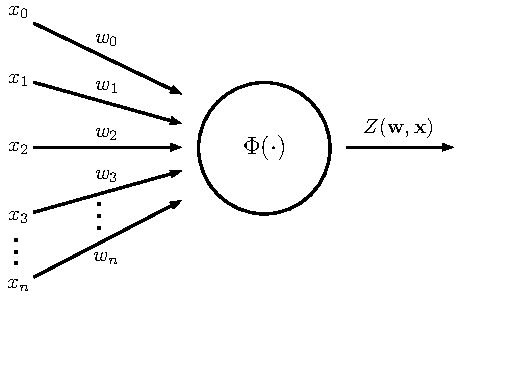
\includegraphics[width=0.5\textwidth]{perceptron}
	\caption{Complete Perceptron Mathematical Model.}
	\label{fig:perceptron}
\end{figure}



\subsection{Multi Layer Perceptron}\label{sec:MLP}

\subsection{Backpropagation}\label{sec:backpropagation}

\section{Acoustic Emission}\label{sec:acousticEmission}

\section{Bibliography Review} \label{sec:bibliographyReview}